\documentclass[FM,BP]{tulthesis}
% tento dokument používá balíky specifické pro XeLaTeX a lze jej přeložit jen XeLaTeXem.

% ENGLISH EXPLANATION
% \documentclass[FM,Dis,EN,fonts,bw]{tulthesis} % black and white typing, dissertation thesis at FM, written in English with using of TUL Mono font
% this document uses packages specific for XeLaTeX and it is possible to 
% compile it by XeLaTeX only, if you haven't installed used (commercial) fonts
% change them or erase commands \set...font in following rows
% settings: FM (faculty: FS, FT, FP, EF, FA, FM, FZS a CXI), Dis (type of thesis: BP, DP, Teze, Autoref, Hab, SP, Proj), EN (written in English language), fonts (activation of TUL fonts), bw (black and white)

% Autor of the template tulthesis: Pavel Satrapa: http://www.nti.tul.cz/~satrapa/vyuka/latex-tul/

% Autor of several comments and their translation into English, BibLaTeX settings and CSN ISO 960 citation standard setting: Jan Koprnický
% http://www.fm.tul.cz/personal/jan.koprnicky

\newcommand{\verze}{2.0}

% školní balíčky
\usepackage{polyglossia}
\setdefaultlanguage{czech}

\usepackage{makeidx}
\makeindex

\usepackage{xunicode}
\usepackage{xltxtra}

% příkazy specifické pro tento dokument / specific commands for this document
\newcommand{\argument}[1]{{\ttfamily\color{\tulcolor}#1}}
\newcommand{\argumentindex}[1]{\argument{#1}\index{#1}}
\newcommand{\prostredi}[1]{\argumentindex{#1}}
\newcommand{\prikazneindex}[1]{\argument{\textbackslash #1}}
\newcommand{\prikaz}[1]{\prikazneindex{#1}\index{#1@\textbackslash #1}}
\newenvironment{myquote}{\begin{list}{}{\setlength\leftmargin\parindent}\item[]}{\end{list}}
\newenvironment{listing}{\begin{myquote}\color{\tulcolor}}{\end{myquote}}
\sloppy

% deklarace pro titulní stránku / title page declaration
\TULtitle{Návrh jádra procesoru architektury RISC-V v FPGA}{ RISC-V architecture based processor core in an FPGA}
\TULauthor{Jaroslav Körner}

% pro bakalářské, diplomové a disertační práce / for bachelor, master theses and dissertation
\TULprogramme{B0613A140005}{Informační technologie}{Information technology}
\TULbranch{}{Inteligentní systémy}{Intelligent systems}
%\TULbranch{1802T008}{Nějaký jiný obor}{Some other branch}
\TULsupervisor{Ing. Martin Rozkovec, Ph.D.}
\TULyear{2023}

% Použití bibLateXu, pracuje s ISO stylem
% BibLaTeX settings, works with ISO style
\usepackage[ 
    backend=biber
    % ,style=iso-authoryear % styl vyžaduje FZS TUL , místo příkazu \cite{} je potřeba využít \parencite{} (sazba kulatých závorek) / style required by FZS TUL use \parencite{} instead of \cite{}
    ,style=iso-numeric
    %,style=numeric
    %,sortlocale=cs_CZ
    ,autolang=other
    ,bibencoding=UTF8
    %,urldate=edtf
    ,maxcitenames=2 %maximum v textu citovaných jmen
    ,maxbibnames=3 %maximum v seznamu vyjmenovaných autorů
    ]{biblatex}
\addbibresource{arefBP_RISC-V.bib}% vložení seznamu literárních zdrojů v bib formátu / input of references in bib format

% Úprava iso-numeric.bbx v souladu s požadavky TUL hranaté závorky v číslovaném seznamu / Modification of iso-numeric.bbx in accordance with TUL requirements of square brackets in a numbered list
\DeclareFieldFormat{labelnumberwidth}{\mkbibbrackets{#1}}

% Formátování podle pokynů FZS, při využití stylu iso-authoryear, čárka mezi jmény a poslední jméno se spojkou a / special requirements of FZS TUL 
\DeclareDelimFormat{multinamedelim}{\addcomma\space}

\DeclareDelimFormat{finalnamedelim}{%
  \ifnumgreater{\value{liststop}}{2}{\finalandcomma}{}%
  \addspace\bibstring{and}\space}

\DeclareNameAlias{author}{family-given/given-family} 
%%%%%%%%%%%%%%%%%%%%%%%%%%

\usepackage{csquotes} %užití biblatexu hlasí warnings, důvodem může být použití českých uvozovek v citacích! / solving of problems with Czech quotations
\urlstyle{same} %sazba url odkazů stejným fontem jako ostatní text, řešení problémů v zalamování hypertextových odkazů v citacích / url in references setting into the same form as text 


% přidané balíčky
\usepackage{multirow}
\usepackage{pdfpages}
\usepackage{amsmath}
\usepackage{bigfoot}
\usepackage{minted}
\usepackage{xparse}
\usepackage{tikz}
\usepackage{svg}

\usetikzlibrary{shapes,arrows}

\let\oldquote\quote
\let\endoldquote\endquote

\RenewDocumentEnvironment{quote}{om}
  {\oldquote}
  {\par\nobreak\smallskip
   \hfill(#2\IfValueT{#1}{~---~#1})\endoldquote 
   \addvspace{\bigskipamount}}

% začátek dokumentu
\begin{document}

%\ThesisStart{male}
%\ThesisStart{zadani-a-prohlaseni.pdf}
\ThesisStart{assets/BP_JK_zadani.pdf}

\begin{abstractCZ}
Tato bakalářská práce se zabývá návrhem jedno jádrového procesoru architektury RISC-V32I, tedy procesoru s 32 bitovou adresací paměti pracující nad datovým typem integer. Návrh byl omezen na neprivilegovaný instrukční soubor. 
Jádro procesoru je navrženo v jazyce VHDL. Tento návrh byl následně otestován pomocí simulace v prostředí Xilinx Vivado. Celková funkčnost je předvedena jednoduchým demonstračním programem spuštěným na desce Avnet ZedBoard.
\end{abstractCZ}

\begin{keywordsCZ}
bakalářská práce, 32-bitový mikroprocesor,  architektura instrukčního souboru RISC-V32I, návrh hardwaru v jazyce VHDL, programovatelné hradlové pole
\end{keywordsCZ}

\vspace{2cm}

\begin{abstractEN}
This bachelor thesis deals with a design of a single-core processor of the RISC-V32I architecture, i.e. a processor with 32-bit memory addressing and working over the integer data type. The design was limited to unprivileged instruction set.
The processor core is designed in the VHDL language. This finished design has been tested using simulation in Xilinx Vivado environment. The overall functionality is demonstrated by a simple demonstration program running on the Avnet ZedBoard.
\end{abstractEN}

\begin{keywordsEN}
bachelor thesis, 32-bit microprocessor, RISC-V32I instruction set architecture, hardware design in VHDL, field programmable gate array
\end{keywordsEN}

\clearpage

\begin{acknowledgement}
Rád bych poděkoval mým učitelům ze střední školy, kteří mne zasvětili do zázraků a tajů číslicové techniky. Také pedagogickému kolektivu na ČVUT, kteří mi ukázali základy návrhu architektury procesorů typu MIPS v předmětu APO. Dále chci poděkovat Ing.\,Martinu Rozkovcovi, Ph.D., jenž se odhodlal být vedoucím mé bakalářské práce, za to, že za celou tu dobu nade mnou nezlomil hůl i když stále zůstávám v srdci programátor a nikoliv architekt. 

\end{acknowledgement}

\tableofcontents

\listoffigures

\listoftables

\renewcommand\listoflistingscaption{Seznam zdrojových kódů}
\listoflistings

\clearpage

\begin{abbrList}
    \textbf{ALU} & Aritmeticko-Logická Jednotka \\
    \textbf{ARM} & Advanced RISC Machine / Acorn RISC Machine \\
    \textbf{AXI} & Advanced eXtensible Interface \\
    \textbf{ce} & clock enable \\
    \textbf{CPU} & Central Processing Unit \\
    \textbf{CISC} & Complex Instruction Set Computer \\
    \textbf{CU} & Control Unit \\
    \textbf{DSP} & digital signal procesing \\
    \textbf{FPGA} & Field Programmable Gate Array \\
    \textbf{GNU} & GNU's Not Unix! \\
    \textbf{HW} & Hardware \\
    \textbf{IDE} & integrated development environment \\
    \textbf{ISA} & Instruction Set Architecture \\
    \textbf{LUT} & look up table \\
    \textbf{MMAP} & memory mapped device \\
    \textbf{NOP} & no operation \\
    \textbf{PC} & Program Counter \\
    \textbf{RISC} & Reduced Instruction Set Computer \\
    \textbf{RISC-V} & Reduced Instruction Set Computer - Version 5 (čti: risk pět) \cite{RISC-V_meaning}\\
    \textbf{rd} & Register Destination \\
    \textbf{rs1} & Register Source 1 \\
    \textbf{rs2} & Register Source 2 \\
    \textbf{SoC} & system on chip \\
    \textbf{SW} &  Software \\
    \textbf{VHDL} & Very High Speed Integrated Circuit Hardware Description Language \\
    \textbf{WSL} & Windows Subsystem for Linux \\
    \textbf{XLEN} & šířka registrů procesoru \\
    \textbf{XPM} & Xilinx Parameterized Macros
\end{abbrList}\clearpage

\chapter{Předmluva}
Jistě se ptáte, co stálo za mým rozhodnutím zvolit si za téma mé bakalářské práce návrh vlastního procesoru?

Již na střední škole ve mne vzbudil velký zájem předmět číslicové technologie a vše s ním spojené. Když jsem poprvé za sebe zapojil čtyři čtyřbitové inkrementální čítače 7493 \cite{wiki_7400} s příslušnými moduly 24,10,6,10. Čtyři dekodéry na 7-segment 7449 a za ně odpory a displeje. Tuto hromadu švábů a propojovacích vodičů jsem napojil na generátor hodinového signálů (předpokládám značky Tesla), tak se před mým zrakem rozeběhly číslíčka primitivních digitálních hodin. V tu chvíli se mi rozzářily oči a já měl pocit, jako že jsem právě v tom okamžiku ovládl tranzistory a elektrický proud.

Netrvalo to dlouho a naskytla se mi příležitost rozebrat svůj první stolní počítač (těmito slovy myslím kamarádův). Vypojil jsem ho ze zásuvky a s křížovým šroubovákem v jedné ruce jsem hbitě postupoval skříní k jeho niternějším a niternějším útrobám. Nakonec již nezbylo nic, co bych mohl z šasi vyjmout. Rozprostíral se zde přede mnou na kuchyňském linoleu úplně nový svět. Svět plný prapodivných součástek a elektroniky, které bych si dříve nedovedl představit ani v těch nejdivočejších snech. Při kompletaci jsem pokračoval v opačném pořadí, než při demontáži a když má práce ustala, stál zde opět více méně, až na pár šroubků, ten původní počítač. Stačilo ho už jen zapnout. Mé srdce se rozbušilo. Spatřil jsem však ještě jedno tlačítko vzadu na zdroji počítače, které jsem řádně neprozkoumal. Věděl jsem, že musím stůj co stůj přijít na to, co se stane, když ho přepnu. Učinil jsem tak a ozvala se rána, jako když střelí z děla a z útrob počítače se vyvalil začernalý obláček dýmu. 

V tu chvíli jsem měl jasno. Ten den na tom místě jsem se zapřisáhl, že neustanu ve svém bádání, dokud neodhalím všechna kouzla, čáry a taje, které v sobě počítačová skříň skrývá. 

Tyto a další události vedly k tomu, že dnes stojím právě zde a jsem rozhodnut navrhnout si svůj vlastní procesor. 

\chapter{Úvod}
Tato bakalářská práce se zabývá vytvořením návrhu procesoru RISC-V32I ve VHDL\index{VHDL}. Jedním ze základních úkolů této bakalářské práce je seznámení se podrobněji s architekturou procesorů RISC-V. 

Cílem bylo popsat návrh procesoru s jedním jádrem, který je vybaven 32 bitovou adresní sběrnicí. Procesor disponující aritmetickologickou jednotkou, která umožňuje sčítání, odčítání a všechny základní operace booleovské algebry nad celými čísly. Procesor bude omezen pouze na neprivilegovaný instrukční soubor.
Jednotlivé části návrhu procesoru budou otestovány simulací v prostředí Xilinx Vivado. Poté co bude procesor plně navržen, projde všemi simulacemi a úspěšnou syntézou, tak dojde k jeho nahrání na vývojovou desku Avnet ZedBoard. Po nahrání do FPGA na něm bude ověřena jeho funkčnost pomocí demonstračního programu, jenž otestuje procesor při ovládaní vstupních a výstupních periferií. 

Kapitola \ref{kap:teorie_cpu} Důležité body teorie návrhu procesorů na straně \pageref{kap:teorie_cpu} seznámí čtenáře se základním dělením architektur počítačů a procesorů.

Kapitola \ref{kap:RISC-V} s názvem RISC-V na straně \pageref{kap:RISC-V} se zabývá obsahem anglické specifikace architektury RISC verze pět z roku 2019 dostupné na webu \href{https://riscv.org/wp-content/uploads/2019/12/riscv-spec-20191213.pdf}{\emph{riscv.org}}, v souladu s kterou je tento procesor navržen. Kapitola je rozdělena do sekcí podle logického dělení instrukčního souboru.

Kapitola \ref{kap:Návrh procesoru} Návrh procesoru je rozdělena do sekcí tak, aby jejich pořadí korespondovalo s postupnými kroky návrhu částí procesoru. 

Kapitola \ref{kap:Programy} Programy čtenáře nejprve seznámí s krátkým úvodem pro programování v jazyce symbolických adres. Dále se věnuje překladu zdrojových kódu a jejich nahrání do navrženého procesoru.

\paragraph{}
Všechny soubory návrhu a programy jsou dostupné v repositáři GitLabu\footnote{Pro přístup je nutné použít VPN do sítě TUL.} na adrese: 
\href{https://gitlab.tul.cz/jaroslav.korner/RISC-V/}{\emph{https://gitlab.tul.cz/jaroslav.korner/RISC-V/}} 

\chapter{Důležité body teorie návrhu procesorů} \label{kap:teorie_cpu}

\section{Architektura procesoru}
Teď již k samotnému návrhu procesoru, ale kde začít? Asi nejstěžejnějším rozhodnutím před tím, než člověk vůbec začne něco navrhovat, je rozhodnout se, jakou použije architekturu a instrukční sadu s ní spojenou. Za základní dělbu architektur lze považovat RISC a CISC. 

\subsection{CISC} \label{kap:CISC}
Hlavní rodinou procesorů z vývojové větve CISC je bez pochyby 32bitová x86 \cite{8086} od \href{https://www.intel.com/content/www/us/en/homepage.html}{\emph{Intelu}} z něj odvozená architektura AMD64 \cite{AMD64}, ke které \href{https://www.amd.com/en}{\emph{AMD}} přidalo 64bitovou podporu.

Traduje se že inženýři v Intelu pracovali dlouhý čas na průlomovém procesoru, který by svými moderními vlastnostmi a bezpečným přístupem na prvním místě vytřel zrak konkurenci. AMD jim však dýchalo na paty a tak v oddělení vedení na velitelství Intelu rozhodli udělat radikální krok a za pouhých čtrnáct dní představit svůj zbrusu nový procesor. Ve vývoji z toho nebyli nadšení a věděli že stojí před nemožným termínem a proto se rozhodli upustit od svého dlouho piplaného projektu a ve zbývajícím čase navrhnout něco sice mnohem méně ambiciózního, ale taky nového lepšího než má konkurence. 

Nakonec z nich vypadl procesor 8086 s 8 16-bitovými registry (kde 4 jdou rozdělit každý na dva 8bitové). Ten byl kompatibilní se svými předchůdci a dával velký důraz na práci s pamětí přes stack\index{stack} (tedy potřebu sáhnout na pamět RAM\index{RAM} pokaždé když chce další číslo), nikoliv registry jako takovými. Zpětně jim to nelze dávat za zlé, 16bitů opravdu není mnoho, když tam chcete nacpat adresy operandů a k ním ještě operaci jako takovou. Cena přidání registrů byla vysoká a připojovaná datová média byla zoufale pomalá, takže při nízké frekvenci na které tehdejší procesory pracovali to vyšlo prašť jak uhoď. Intel s vývojem svých procesorů přidával složitější instrukce, které stále pracovaly s daty uloženými přímo v paměti. Když se procesory zrychlili pomocí zřetězeného zpracování a lepšímu výrobnímu procesu s menšími tranzistory, začala se prohlubovat propast mezi vybavovacími časy paměti RAM a taktem jádra procesoru. Nač počítat velmi rychle, když nemáte s čím? K procesorům se začala přidávat takzvaná vyrovnávací paměť cache, rychlejší než RAM, ale levnější než registry. Její hlavní výhoda tkvěla v tom že nemusíte měnit instrukční sadu. S komplexitou instrukcí také narostla spotřeba procesoru, protože je jedno že danou operaci zrovna nepoužíváte, ale ten křemík co jí tvoří musíte stejně vyrobit a živit už ho napořád.

Nevýhoda architektury x86 co se týče vlastního návrhu je v tom, že vám k tomu Intel nedá své požehnání \cite{wiki_X86}.

\subsection{RISC} \label{kap:RISC}
Ze zdejší rodiny se asi do nedávna nejhlasitěji ozýval \href{https://www.arm.com}{\emph{ARM}}. Tato architektura byla vytvořena na Univerzitě v Cambridge \cite{Kumarsahoo472022} aby učitelé na předmětu Architektura procesorů měli o čem přednášet, jelikož x86/AMD64 je již v dnešní době příliš komplikovaná a o licenci pro návrh se dělí jen pár firem. Jiné jednoduší architektury povětšinou zastaraly a pohltil je čas, takže se nehodili pro demonstraci moderních přístupů návrhu procesorů. 
Nevýhoda procesorů ARM je pro nás v tom, že ten kdo je chce vyrábět či navrhovat musí zaplatit tučnou licenci \cite{ARM_licence}.

Za zmínku též stojí MIPS od \href{https://www.mips.com/}{\emph{MIPS Technologies}}, který byl vznikl na univerzitě ve Stanfordu \cite{Mips} jako výukový projekt vedený Johnem Hennessey. Ač jsou i tyto procesory vyráběny, tak se na trhu zdaleka neuchytili natolik jako ARM.

\href{https://www.sifive.com}{\emph{RISC}} dělá věci jinak. Jde o mnohem modernější přístup. Procesor disponuje značným počtem registrů (běžně 32 u 32bitových procesorů), při volání jednodušších funkcí není třeba plnit stack\index{stack}, ale stačí využít k tomu vyhrazených registrů (což je rychlejší). Pro přístup do paměti lze běžně použít pouze instrukce \textbf{LOAD} a \textbf{STORE}. Jde o menší, lehčí a pružnější návrh, který se snažil začít s čistým štítem a osekat přebytečný křemík, tak aby vznikla vysoká účinnost na watt i za cenu menšího počtu provedených instrukcí na takt ve srovnání architekturou CISC \cite{wiki_RISC}.

Jednou z mladších větví je \href{https://en.wikipedia.org/wiki/RISC-V}{\emph{RISC-V}}, který vznikl na Univerzitě v Californii, Berkeley pod vedením Davida Pattersona. Tato architektura je dnes pod open source licencí. Tam kde ARM licencuje svá jádra pro výrobu či modifikaci, tak RISC-V\index{RISC-V} volně nabízí instrukční sady, které můžete použít k vývoji vašeho procesoru \cite{RISC-V_history}. Této architektuře je věnována stále větší pozornost i na poli velkých hráčů jako jsou:  
\href{https://pathfinder.intel.com}{\emph{Intel}},
\href{https://circuitcellar.com/newsletter/amd-is-hiring-risc-v-cpu-developers/}{\emph{AMD}} či
\href{https://www.sifive.com/press/nasa-selects-sifive-and-makes-risc-v-the-go-to-ecosystem}{\emph{NASA}}.

Spoustu nových projektů vzniká právě nad touto architekturou:
nejrychlejší RISC-V procesor
\href{https://www.cnews.cz/zatim-nejrychlejsi-procesor-risc-v-na-svete-vyrabi-ho-intel-na-4nm-procesu-umi-pcie-5-0-i-ddr5/}{\emph{zde}}, první notebook s procesorem RISC-V
\href{https://www.tomshardware.com/news/risc-v-laptop-world-first}{\emph{zde}},
Raspberry Pi klon
\href{https://www.czc.cz/radxa-rock-4-se-4gb/359880/produkt?gclid=Cj0KCQiAi8KfBhCuARIsADp-A54p9OKqDmKCbrRN9vUVP0A1xcUF1QDlwx-Gjsei9Vh2oUKDrGFNSIcaAoffEALw_wcB}{\emph{zde}}.

\paragraph{}
Právě z důvodu otevřené licence a aktuálnosti jsem se rozhodl použít pro svůj návrh procesoru architekturu RISC-V.

\subsection{Současnost}
V dnešní době se rozdělení na CISC a RISC rozmazává. Procesory s architekturou CISC jsou vnitřně postavené na rozkladu instrukcí na mikrokód, který se svým vykonáváním již podobá operacím tak typickým pro architektury typu RISC.
Naopak instrukční sada procesorů RISC je rozšiřována o instrukce (SIMD) pro práci s vektory a multimediální operace, které svými vlastnostmi splňují charakteristiku přístupu CISC. 

\newpage
\section{Schéma počítače}
Na procesory lze také nahlížet z pohledu jak pracují s pamětí. Existují dva směry přístupu, Von Neumanovo a Harvardské schéma počítače. 

\subsection{Harvardské schéma počítače} \label{kap:Harvardské schéma počítače}
Harvardská architektura byla navržena Howardem Aikenem na Harvardské univerzitě ve třicátých letech dvacátého století. Na této architektuře byl postaven například počítač ENIAC. Vyznačuje se tím, že má oddělenou instrukční a datovou paměť \cite{Kuty2014}. 

\begin{figure}[h]
    %\includegraphics[width=\textwidth]
    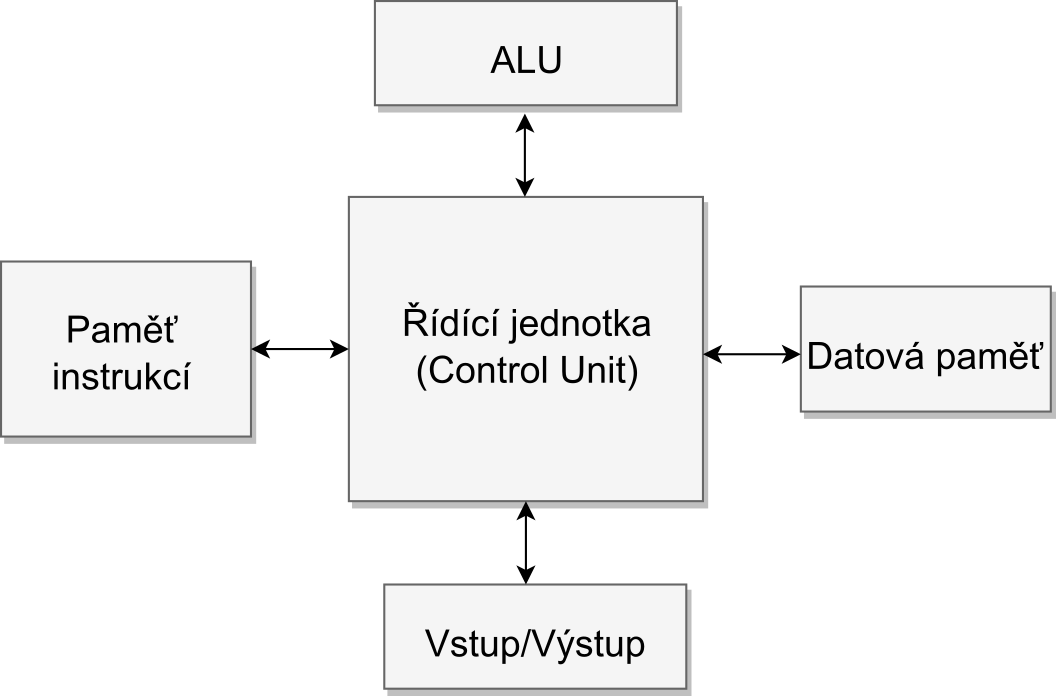
\includegraphics[scale=1]{assets/Harvard_Architecture.png}
    \centering
    \caption{Harvardské schéma (převzato z \cite{Schema_pc})}
    \label{img:Harvard}
\end{figure}

\paragraph{}
Mezi výhody, které tento přístup přináší, lze zařadit například:
\begin{itemize}
    \item Větší propustnost při komunikaci (najednou lze načítat z paměti jak data, tak i příští instrukci).
    \item Paměť může využívat různé technologie (instrukční PROM, datová RAM).
    \item Instrukční paměť je chráněna proti nechtěnému zápisu. 
\end{itemize}

\paragraph{}
Mezi nevýhody patří:
\begin{itemize}
    \item Nemožnost změnit program za běhu.
    \item Architektura může mít větší požadavky na paměť oproti Von Neumannově. 
    \item Architektura má zvýšenou komplexitu návrhu přidanou sběrnicí. \cite{gfg_harvard}
\end{itemize}

\subsection{Von Neumanovo schéma počítače} \label{kap:Von Neumanovo schéma počítače}
Svůj název schéma získalo podle autora přednášky „First Draft of a Report on the EDVAC“ Johna von Neumanna \cite{First_Draft}. Jde o jednoduché schéma počítače, kdy jsou instrukce procesoru i data ke zpracování uložena v jedné paměti přistupované po společné sběrnici. Nelze tedy najednou načítat jak program tak data a sběrnice do operační paměti se stává úzkým místem. \cite{VNEUM}

\begin{figure}[h]
    %\includegraphics[width=\textwidth]
    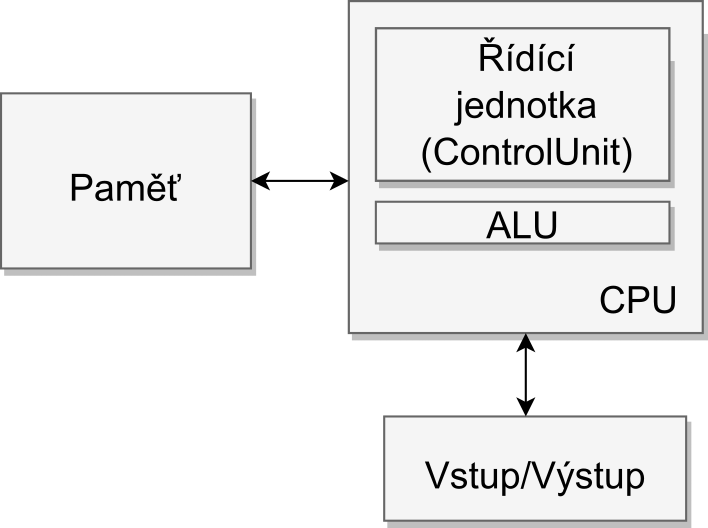
\includegraphics[scale=1]{assets/Von_Neumann_Architecture.png}
    \centering
    \caption{Von Neumannovo schéma (převzato z \cite{Schema_pc})}
    \label{img:VonNeumann}
\end{figure}

\paragraph{}
Návrh popisoval počítač skládající se z těchto částí:
\begin{itemize}
    \item \textbf{Operační paměť} ukládá všechna data,
    \item \textbf{ALU} provádí aritmetické a logické operace,
    \item \textbf{Řídící jednotka} která určuje co se má v danou chvíli vykonávat,
    \item \textbf{Vstupní zařízení} slouží pro komunikaci s vnějším světem,
    \item \textbf{Výstupní zařízení} slouží pro komunikaci s vnějším světem.
\end{itemize}

\newpage
\subsection{Současnost}
V praxi mají počítače mezi procesorem a operační paměti ještě mezistupeň, kterým je asociativní paměť (cache\index{cache}, i ta je dnes víceúrovňová). Přístup do paměti je násobně pomalejší než vykonávání základních aritmetických operací na procesoru a tak do hry vstoupila výše zmíněná asociativní paměť, malá a rychlá paměť, která umožňuje zrychlení opakovaného přístup na stejná data či instrukce (ty jsou vícekrát po sobě načítány zejména v cyklech). Asociativní paměť dnes bývá rozdělena na instrukční a datovou. Tak vzniká hybridní návrh. Procesor může nezávisle přistupovat ke svým instrukcím a datům (dokud jsou načtené v asociativní paměti), zatímco z procesoru ven vede do operační paměti jen jedna datová sběrnice \cite{wiki_Von_Neumannova_architektura}.

\newpage
\section{Organizace paměti programu} \label{kap:Organizace paměti programu}

Operační paměť v procesoru lze z pohledu spuštěné aplikace rozdělit na tyto části: 
\begin{itemize}
    \item \textbf{Zásobník}: obsahuje lokální proměnné funkcí
    \item \textbf{Halda}: dynamicky alokovanou paměť
    \item \textbf{Data}: globální proměnné
    \item \textbf{Text}: obsahující spuštěný program
\end{itemize}

Na obrázku \ref{img:StackAndHeap} je vyobrazeno jak jsou tyto segmenty paměti poskládány. Na nejnižší adrese začíná segmentem text, následují ji data a halda se zásobníkem, které se opticky dělí o jeden společný prostor. \cite{courses_Stack_and_Heap}

\begin{figure}[h]
    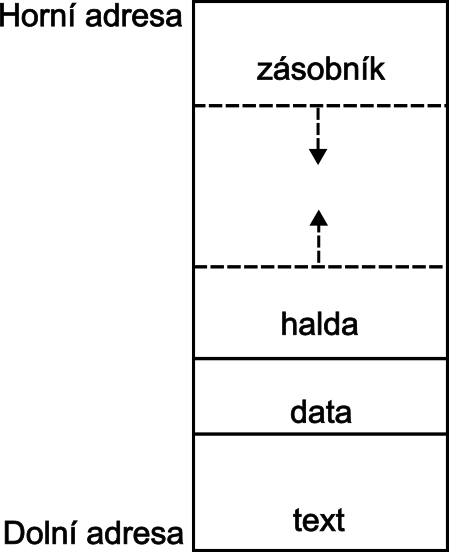
\includegraphics[scale=0.5]{assets/Stack.png}
    \centering
    \caption{Segmenty paměti (překresleno podle \cite{courses_Stack_and_Heap})}
    \label{img:StackAndHeap}
\end{figure}

\subsection{Text} \label{kap:Text}
Segment text začíná od adresy 0x00000000\footnote{0x značí zápis v šestnáctkové soustavě.} (32b), roste směrem nahoru. Je zde uložený program. Při spuštění počítače se čítač programu nastaví na nulu a program se začne vykonávat z této adresy, tedy v sekci text. 

\subsection{Data}
Je sekce ve kterém jsou uložené konstanty programu. Jejich adresa se v průběhu celého programu nemění, zůstávají na jednom místě a díky tomu je možné na ně přistupovat z libovolné části programu, i když se rámec kontextu na zásobníku volně přesouvá. 

\subsection{Halda}
Halda (heap) je nepovinný segment v operační paměti, kam se ukládají rozměrné datové typy (pole, struktury, objekty), se kterými je následně pracováno v programu pomocí reference (v jazyce C ukazatel). Paměťový prostor je zde potřeba pro použití v programu alokovat (dynamická alokace). 

Během překladu lze snadno spočítat velikost staticky alokovaných datových struktur (jak velká jsou například pole), zatímco při dynamické alokaci\footnote{Název je přejat od slova dynamit, u toho taky nikdy nevíte jak velká ta díra bude dokud to nevybouchne.} není při překladu jasné kolik paměti se má vyhradit (vektory, přidání záznamu do spojového seznamu).

Když data uložená v alokovaném prostoru již nejsou potřeba, tak tuto paměť musíme před dalším použitím uvolnit (dealokovat). Při častém vytvářením objektů a jejich uvolňování může dojít k problému fragmentace paměti. To je stav, kdy mezi alokovanými objekty zbývá malý prostor, do kterého se již nová data nevejdou. 

\subsection{Zásobník}
Zásobník (stack) začíná na nejvyšší adrese 0xFFFFFFFF (32b) a roste ze shora dolů. Zásobník obsahuje jednotlivé rámce. Ukazatel na vrchol rámce se standardně ukládá do jednoho z registrů procesoru. Při volání funkce se vytvoří nový rámec o velikost potřebné pro argumenty a lokání proměnné dané funkce (hodnota v registru sp\index{sp} se aktualizuje). Když se z lokálního kontextu volá další funkce, tak zásobník pokračuje v růstu jako krápník od shora dolů. Při návratu z funkce se bloky rámců odmazávají a krápník ustupuje nahoru. 

\newpage
Tento paměťový prostor bývá standardně pro aplikace omezen a tak se velké datové struktury alokují na haldu (heap). Nejkrajnějším omezením zásobníku může být hranice oblasti \textbf{text} ve které je uložen program. Další zápis do zásobníku by vedl k tomu, že by se přepsal spouštěný program a aplikace by již nemohla zaručit své správné vykonání. Tento problém se při detekování běžně označuje za „stack overflow“. \cite{Javatpoint_SackVsHeap}

\begin{figure}[h]
    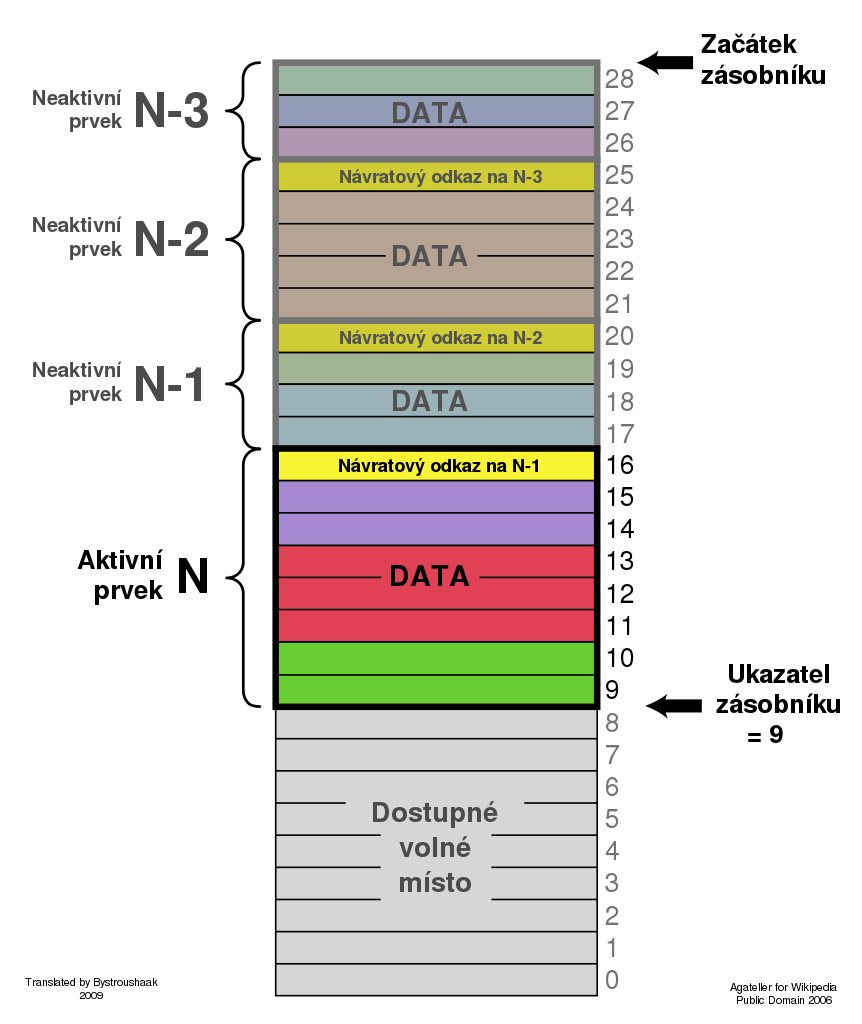
\includegraphics[scale=0.3]{assets/ProgramCallStack.png}
    \centering
    \caption{Zásobník (převzato z \cite{wiki_zasobnik})}
    \label{img:Stack}
\end{figure}

Na obrázku \ref{img:Stack} je vyobrazená sekce zásobník. Velké „N“ značí lokální kontext běžící funkce, „N-1“ je předchozí rámec, ze kterého byla tato funkce zavolána. Řádky značí jednotlivé proměněné délky výchozího slova systému. První řádek rámce obsahuje návratovou adresu do programu předchozí funkce. 

\newpage

\section{Jazyk pro popis hardware}
Jazyk VHDL (Very High Speed Integrated Circuit Hardware Description Language) poskytuje návrhářům hardwaru vyšší úroveň abstrakce než je tomu v metodologii návrhu přes booleovské rovnice a pravdivostní tabulky, ze kterých vzniká schema obvodu, nebo intuitivní schématický návrh s použitím obvodů SSI. To umožňuje díky tomu že vznikl právě za účelem popisu chování integrovaných obvodů. Za tímto jazykem popisující hardware stojí Ministerstvo obrany USA a stal se standardem IEEE. Jeho syntaxe vychází z jazyka ADA. Jde o jazyk silně typový, který vyžaduje použití konverzních funkcí pokaždé když se mění typ signálu. 



Specifikace RISC-V slovně a za pomoci tabulek s kódy operací a vzory instrukcí formalizuje vlastnosti architektury. Díky vlastnostem jazyka VHDL je možné přeložit tuto textovou předlohu do kódu popisujících návrh procesoru. 

\subsection{Strukturní vs behaviorální popis}
Čistě behaviorální popis může krok za krokem popisovat co se má vykonávat při jednotlivých instrukcích. Takovýto postup může být pro člověka čitelnější a jednoduší na tvorbu, jelikož přímo koresponduje s formulaci významu instrukcí ve specifikaci a veškerá zákoutí návrhu potřebná pro pochopení funkce daných instrukcí jsou na jednom místě v programu. 

Nevýhoda takového návrhu je však v menší modularitě, ze které plyne náročnější testování a simulace (test bench). Do budoucna je v plánu rozšířit návrh procesoru RISC-V o zřetězené zpracování instrukcí. To by však bylo v takovém přístupu velmi náročné.  

Zvolil jsem si proto cestu kombinace strukturního a behaviorální popisu. Práce je tak rozdělena do souborů podle jednotlivých logických celků. To umožňuje opakovaného použití HW (entit) na více místech v návrhu. Testování těchto dílčích částí je teoreticky mnohem snazší, protože například ALU nebo dekodér instrukcí je jedním z bloků návrhu. ALU\index{ALU} je tedy možné instancovat zvlášť a otestovat ji podle specifikace chování aritmetiky celých čísel (integer\index{integer}) pro sčítání a odčítání, podobně otestujeme i funkce booleovské algebry. Tyto nezávislé (unit) testy poskytují návrhářovi důvěru v jednotlivé kusy návrh zatímco z nich skládá větší funkční celky. 

\chapter{RISC-V} \label{kap:RISC-V}
Při návrhu procesoru jsem postupoval podle anglické specifikace a tak většina informacím k architektuře procesoru (jako je například význam a formát instrukcí, adresování paměti, skoky v programu a další) je překladem specifikace RISC-V a to verze \href{https://riscv.org/wp-content/uploads/2019/12/riscv-spec-20191213.pdf}{\emph{riscv-spec-20191213}} \cite{RISC-V}.

Ta určuje několik RISC-V ISA základu, které operují nad datovým typem integer\index{integer},  ale liší se šířkou registrů a datové sběrnice. Přehled je znázorněn v tabulce \ref{table:ISA_bitovost}.

\begin{table}[h]
    \caption{Základní ISA RISC-V}
    \label{table:ISA_bitovost}
    \begin{center}
    \begin{tabular}{|c|l|l|}
    \hline
    \textbf{Rozšíření} & \textbf{Bitovost} & \textbf{Datový typ} \\
    \hline
    RV32I & 32 bitů & integer\\
    RV64I & 64 bitů & integer \\
    RV128I & 128 bitů & integer\\
    \hline
    \end{tabular}
    \end{center}
\end{table}

Jsou zde také definovaný i rozšíření ISA, tabulka \ref{table:ISA_extension}, která lze libovolně kombinovat, podle požadovaných vlastností výsledného procesoru.

\begin{table}[h]
    \begin{center}
    \caption{Rozšíření ISA}
    \label{table:ISA_extension}
    \begin{tabular}{|c|l|l|}
    \hline
    \textbf{Rozšíření} & \textbf{Anglicky} & \textbf{Česky} \\
    \hline
    M & Multiplication and Division & Násobení a dělení \\
    A & Atomic instructions & Atomické instrukce \\
    F & Single-Precision Floating-Point & Floating-Point základní přesnost\\
    D & Double-Precision Floating-Point & Floating-Point dvojitá přesnost\\
    Q & Quad-Precision Floating-Point & Floating-Point čtyřnásobná přesnost\\
    C & Compressed & Komprimovaná (16-bitová) \\
    \hline
    \end{tabular}
    \end{center}
\end{table}

\section{RV32I} \label{kap:RV32I}
Tento procesor implementuje instrukční sadu RISC-V32I. Jde o nejzákladnější podmnožinu operací na 32bitovém celočíselném procesoru RISC-V. Má 40 instrukcí (jejichž přehled je uveden v na obrázku \ref{img:RISC-V_insturctions}), ale při jednodušší implementaci lze popsat instrukci ECALL/EBREAK\index{ECALL}\index{EBREAK}\footnote{Instrukce pro exception-call, tedy softwarová přerušení.} pouze jedinou instrukcí SYSTEM. Instrukci FENCE\footnote{Synchronizace zápisu do paměti a propsání z asociativní paměti do RAM\index{RAM}.} lze implementovat jako instrukci NOP\index{NOP}, za cenu ztráty podpory více vláknových aplikací. Tím se sníží rozsah instrukční sady na pouhých 38 instrukcí. 
Programově lze na této ISA emulavot všechny ostatní rozšíření kromě A (atomických instrukcí). 

\begin{figure}[h]
    %\includegraphics[width=\textwidth]
    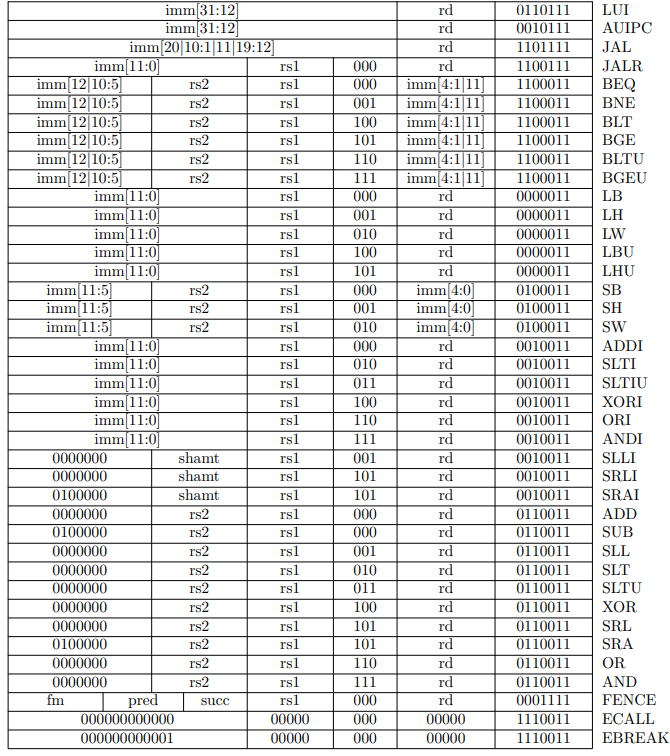
\includegraphics[scale=0.8]{assets/RV32I_instructions_small.png}
    \centering
    \caption{Instrukce ISA RV32I (převzato z \cite{RISC-V})}
    \label{img:RISC-V_insturctions}
\end{figure}

\section{Registry}
V tabulce \ref{table:registers} jsou popsány všechny adresovatelné registry základní neprivilegované ISA. Architektura RV32I má 32 celočíselných registrů, každý 32 bitů široký, tedy XLEN=32\footnote{Terním XLEN značí šířku integerového\index{integer} registru.}. Registr x0 je pevně zapojen všemi svými bity na 0. Obecné registry x1–x31 obsahují hodnoty, které různé instrukce interpretují jako:
\begin{itemize}
    \item kolekci booleovských hodnot,
    \item dvojkový doplněk (znaménková binární celá čísla), 
    \item bezznaménková binární celá čísla.
\end{itemize}

\begin{table}[h]
    \caption{Registry a jejich symbolických pojmenování (převzato z \cite{RISC-V_calling})}
    \label{table:registers}
    \begin{center}
        \begin{tabular}{|l|l|p{4,5cm}|l|}
        \hline
        \textbf{Název registru} & \textbf{Symbolický název} & \textbf{Popis} & \textbf{Ukládá} \\
        \hline
        x0 & zero & Vždy nula & \\
        \hline
        x1 & ra & Návratová adresa & Volající \\
        \hline
        x2 & sp & Ukazatel na stack\index{stack} & Volaný \\
        \hline
        x3 & gp & Globální ukazatel &\\
        \hline
        x4 & tp & Ukazatel na vlákno &\\
        \hline
        x5 & t0 & Dočasný / alternativní návratová adresa & Volající \\
        \hline
        x6–7 & t1–2 & Dočasný & Volající \\
        \hline
        x8 & s0/fp & Ukládaný / ukazatel rámce & Volaný \\
        \hline
        x9 & s1 & Ukládaný & Volaný \\
        \hline
        x10–11 & a0–1 & Argument funkce / návratová hodnota & Volající \\
        \hline
        x12–17 & a2–7 & Argument funkce & Volající \\
        \hline
        x18–27 & s2–11 & Ukládaný & Volaný \\
        \hline
        x28–31 & t3–6 & Dočasný & Volající \\
        \hline
        \end{tabular}
    \end{center}
\end{table}

ISA nespecifikuje který registr musí být použit jako sp\footnote{sp - stack pointer, ukazatel na zásobník} nebo ra\footnote{ra - return address, návratová adresa z funkce}. Mezi osvědčené postupy však patří využívat registr x1 jako návratovou adresu (alternativně x5). Stejně tak registr x2 běžně slouží jako ukazatel na zásobník. Tabulka \ref{table:registers} obsahuje přehled symbolických názvů registrů. Lze je použít při programování v jazyce symbolických adres (assembler), pro tvorbu přehlednějšího kódu a kvalitní překladač provede jejich přeložení na index registru. Tabulka \ref{table:registers} též obsahuje sloupeček „Ukládá“, který značí kdo je zodpovědný za ukládání obsahuje registrů na zásobník a jejich obnovení, před návratem z funkce. 

ISA definuje ještě jeden registr pc\footnote{pc - program counter, neboli čítač programu}, který obsahuje adresu aktuální instrukce, zobrazený v tabulce \ref{table:pc}. 

\begin{table}[h]
    \caption{Registr čítače programu (převzato z \cite{RISC-V})}
    \label{table:pc}
    \begin{center}
        \begin{tabular}{lr}
        XLEN-1 & 0 \\
        \hline
        \multicolumn{2}{|c|}{pc}
        \\
        \hline
        \multicolumn{2}{c}{XLEN}
        \end{tabular}
    \end{center}
\end{table}

\section{Kódování instrukcí} \label{kap:immediate}
ISA RV32I specifikuje čtyři základní instrukční formáty (R/I/S/U), tabulka \ref{table:RISU}. Všechny instrukce mají fixní délku 32 bitů a musí být zarovnány na 4 bajty. 
Pokud při skocích v programu adresa následující instrukce není zarovnána na 4 bajty, IALIGN=32 (bitů)\footnote{Termín IALIGN (měřeno v bitech) používáme k odkazu na omezení zarovnání instrukce adresy, které implementace vynucuje. IALIGN je 32 bitů v základním ISA.}, je generovaná výjimka „instruction-address-misaligned“.
Při dekódování instrukce jejíž opcode nedává smysl je vyvolána výjimka „illegal-instruction“.

\begin{table}[h]
    \caption{Formát kódování instrukcí (převzato z \cite{RISC-V})}
    \label{table:RISU}
    \begin{center}
        \begin{tabular}{lrlrlrlrlrlrl}
        31 & 25 & 24 & 20 & 19 & 15 & 14 & 12 & 11 & 7 & 6 & 0 
        \\
        \cline{0-11}
        \multicolumn{2}{|c|}{func7} & \multicolumn{2}{c|}{rs2} & \multicolumn{2}{c|}{rs1} & \multicolumn{2}{c|}{func3} & \multicolumn{2}{c|}{rd} & \multicolumn{2}{c|}{opcode} & R-typ \\
        \cline{0-11}
        \\
        \cline{0-11}
        \multicolumn{4}{|c|}{imm[11:0]} & \multicolumn{2}{c|}{rs1} & \multicolumn{2}{c|}{func3} & \multicolumn{2}{c|}{rd} & \multicolumn{2}{c|}{opcode} & I-typ \\
        \cline{0-11}
        \\
        \cline{0-11}
        \multicolumn{2}{|c|}{imm[11:5]} & \multicolumn{2}{c|}{rs2} & \multicolumn{2}{c|}{rs1} & \multicolumn{2}{c|}{func3} & \multicolumn{2}{c|}{imm[4:0]} & \multicolumn{2}{c|}{opcode} & S-typ \\
        \cline{0-11}
        \\
        \cline{0-11}
        \multicolumn{8}{|c|}{imm[31:12]} & \multicolumn{2}{c|}{rd} & \multicolumn{2}{c|}{opcode} & U-typ \\
        \cline{0-11}
        \end{tabular}
    \end{center}
\end{table}

Jednotlivé typy instrukcí v tabulce \ref{table:RISU} nesou své jméno podle:
\begin{itemize}
    \item \argument{R-typ} je podle anglického slova \textbf{register} (registr),
    \item \argument{I-typ} je od slova \textbf{immediate} (okamžitý),
    \item \argument{S-typ} je od slova \textbf{store} (ukládat),
    \item \argument{U-typ} je od slova \textbf{upper} (horní) a používá se u instrukcí s 20 bitovými konstantami.
\end{itemize}

Z tabulky \ref{table:RISU} je dále patrné, že instrukce ihned (immediate) se vykonávají s jedním registrem (rs) a hodnotou uloženou přímo v kódu programu (konstantou), výsledek se uloží do cílového registru (rd\index{rd}). Naproti tomu registrové instrukce mají dva operandy uložené ve zdrojových registrech rs1\index{rs1} a rs2\index{rs2}, výsledek operace se opět ukládá do registru rd.
Pozice operandů rs1, rs2 a rd se napříč formáty neliší, což umožňuje jednoduché dekódování instrukcí.

Immediate operandy jsou vždy nejprve znaménkově rozšířeny na délku 32bitů. V tabulce \ref{table:RISU} je imm argument uveden s rozsahem bitů v hranatých závorkách. Například imm[11:0] znamená, že se jedná o 12 bitovou hodnotu, která je znaménkově rozšířena na 32 bitů.
Znaménkové rozšíření je jedna z nejdůležitějších operací na okamžitých instrukcích. V RISC-V je znaménkový bit pro všechny okamžité hodnoty vždy uložen v 31 bitu instrukce, aby znaménkové rozšíření mohlo probíhat paralelně s dekódováním instrukce.

\subsection{Kódování okamžitých instrukcí}
Základní čtyři formáty kódování instrukcí lze rozšířit ještě o formáty (B/J) podle toho jak pracují s okamžitou hodnotou, tabulka \ref{table:immediate_encoding}. 

\begin{table}[h]
    \begin{center}
    \caption{Formát kódování immediate\index{immediate} operací (převzato z \cite{RISC-V})}
    \label{table:immediate_encoding}
    \scalebox{0.85}{
        \begin{tabular}{lcrlcrlrlrlcrlrl}
        31 & 30 & 25 & 24 & 21 & 20 & 19 & 15 & 14 & 12 & 11 & 8 & 7 & 6 & 0 
        \\
        \cline{0-14}
        \multicolumn{3}{|c|}{func7} & \multicolumn{3}{c|}{rs2} & \multicolumn{2}{c|}{rs1} & \multicolumn{2}{c|}{func3} & \multicolumn{3}{c|}{rd} & \multicolumn{2}{c|}{opcode} & R-typ \\
        \cline{0-14}
        \\
        \cline{0-14}
        \multicolumn{6}{|c|}{imm[11:0]} & \multicolumn{2}{c|}{rs1} & \multicolumn{2}{c|}{func3} & \multicolumn{3}{c|}{rd} & \multicolumn{2}{c|}{opcode} & I-typ \\
        \cline{0-14}
        \\
        \cline{0-14}
        \multicolumn{3}{|c|}{imm[11:5]} & \multicolumn{3}{c|}{rs2} & \multicolumn{2}{c|}{rs1} & \multicolumn{2}{c|}{func3} & \multicolumn{3}{c|}{imm[4:0]} & \multicolumn{2}{c|}{opcode} & S-typ \\
        \cline{0-14}
        \\
        \cline{0-14}
        \multicolumn{1}{|c|}{imm[12} & \multicolumn{2}{c|}{imm[10:5]} & \multicolumn{3}{c|}{rs2} & \multicolumn{2}{c|}{rs1} & \multicolumn{2}{c|}{func3} & \multicolumn{2}{c|}{imm[4:1]} & \multicolumn{1}{c|}{imm[11]} & \multicolumn{2}{c|}{opcode} & B-typ \\
        \cline{0-14}
        \\
        \cline{0-14}
        \multicolumn{10}{|c|}{imm[31:12]} & \multicolumn{3}{c|}{rd} & \multicolumn{2}{c|}{opcode} & U-typ \\
        \cline{0-14}
        \\
        \cline{0-14}
        \multicolumn{1}{|c|}{imm[20} & \multicolumn{4}{c|}{imm[10:1]} & \multicolumn{1}{c|}{imm[11]} & \multicolumn{4}{c|}{imm[19:12]} & \multicolumn{3}{c|}{rd} & \multicolumn{2}{c|}{opcode} & J-typ 
        \\
        \cline{0-14}
        \end{tabular}
    }
    \end{center}
\end{table}

Jediný rozdíl mezi formáty S a B je v tom, že 12bitové pole bitů okamžité hodnoty se používá k zakódování větvení v násobcích 2 v B formátu. Místo toho, aby se všechny bity v okamžitém kódování instrukce posunuly vlevo o jeden bit v hardwaru, jak je obvyklé, zůstávají střední bity (imm[10:1]) a znaménkový bit na pevných pozicích, zatímco nejnižší bit ve formátu S (inst[7]) kóduje bit vyššího řádu ve formátu B.

Podobně jediný rozdíl mezi formáty U a J je v tom, že 20bitové pole bitů okamžité hodnoty se posune vlevo o 12 bitů, aby vytvořilo konstantu u typu U a o 1 bit, aby vytvořilo konstantu typu J. Umístění instrukčních bitů okamžité hodnoty v U a J formátech je vybráno tak, aby se maximalizoval překryv s ostatními formáty a mezi sebou.

Tabulka \ref{table:sign_extend} ukazuje okamžité hodnoty vytvořené ze všech základních instrukčních formátů a je označena tak, aby ukázala, který bit instrukce (inst[y]) produkuje jaký bit okamžité hodnoty. Například okamžitá hodnota pro formát I je vytvořena z inst[31:20], zatímco okamžitá hodnota pro formát S je vytvořena z inst[31:25] a inst[11:7].

\begin{table}[h]
    \begin{center}
    \caption{Znaménkové rozšíření immediate\index{immediate} instrukcí (převzato z \cite{RISC-V})}
    \label{table:sign_extend}
    \scalebox{0.9}{
        \begin{tabular}{llrlrrlrlrcl}
        31 & 30 & 20 & 19 & 12 & 11 & 10 & 5 & 4 & 1 & 0 
        \\
        \cline{0-10}
        \multicolumn{6}{|c|}{-- inst[31] --} & \multicolumn{2}{c|}{inst[30:25]} & \multicolumn{2}{c|}{inst[24:21]} & \multicolumn{1}{c|}{inst[20]} & I-okamžité \\
        \cline{0-10}
        \\
        \cline{0-10}
        \multicolumn{6}{|c|}{-- inst[31] --} & \multicolumn{2}{c|}{inst[30:25]} & \multicolumn{2}{c|}{inst[11:8]} & \multicolumn{1}{c|}{inst[7]} & S-okamžité \\
        \cline{0-10}
        \\
        \cline{0-10}
        \multicolumn{5}{|c|}{-- inst[31] --} & \multicolumn{1}{c|}{inst[7]} & \multicolumn{2}{c|}{inst[30:25]} & \multicolumn{2}{c|}{inst[11:8]} & \multicolumn{1}{c|}{0} & B-okamžité \\
        \cline{0-10}
        \\
        \cline{0-10}
        \multicolumn{1}{|c|}{inst[31]} & \multicolumn{2}{c|}{inst[30:20]} & \multicolumn{2}{c|}{inst[19:12]} & \multicolumn{6}{c|}{-- 0 --} & U-okamžité \\
        \cline{0-10}
        \\
        \cline{0-10}
        \multicolumn{3}{|c|}{-- inst[31] --} & \multicolumn{2}{c|}{inst[19:12]} & \multicolumn{1}{c|}{inst[20]} & \multicolumn{2}{c|}{inst[30:25]} & \multicolumn{2}{c|}{inst[24:21]} & \multicolumn{1}{c|}{ 0 } & J-okamžité \\
        \cline{0-10}
        \end{tabular}
    }
    \end{center}
\end{table}


\section{Instrukce celočíselných operací}
Základní aritmeticko-logické operace jsou rozdělené do dvou prakticky totožných skupin: registrových (registr\index{registr}) a bezprostředních/okamžitých (immediate\index{immediate}). 

Bezprostřední operace (immediate) jsou operace, které provádíme nad jedním registrem a konstantou (register-immediate), a jsou zakódovány pomocí formátu typu I. Patří sem například instrukce: \argumentindex{ADDI}, \argumentindex{SLTI}, \argumentindex{SLTIU}, \argumentindex{XORI}, \argumentindex{ORI}, \argumentindex{ANDI}, \argumentindex{SLLI}, \argumentindex{SRLI}, \argumentindex{SRAI}. 

Registrové operace (register) jsou operace, které provádíme nad dvěma registry (register-register), a jsou zakódovány pomocí formátu typu R. Patří sem například instrukce: \argumentindex{ADD}, \argumentindex{SUB}, \argumentindex{SLL}, \argumentindex{SLT}, \argumentindex{SLTU}, \argumentindex{XOR}, \argumentindex{SRL}, \argumentindex{SRA}, \argumentindex{OR}, \argumentindex{AND}. 

Registr rd\index{rd} je vždy cílovým registrem.

\subsection{Přetečení při aritmetických operacích}
Součástí základní sady instrukcí není speciální podpora instrukcí pro kontrolu přetečení při celočíselných aritmetických operacích, protože mnoho kontrol přetečení lze levně implementovat pomocí instrukcí větvení. Kontrola přetečení pro neznaménkový součet vyžaduje pouze jednu další instrukci větvení: \verb|add t0, t1, t2; bltu t0, t1, overflow|. Pro znaménkový součet, pokud je znaménko jednoho operandu známo, vyžaduje kontrola přetečení po součtu pouze jednu instrukci větvení: \verb|addi t0, t1, +imm; blt t0, t1, overflow|. To pokrývá běžný případ sčítání s okamžitým operandem. Pro obecný znaménkový součet jsou po součtu vyžadovány tři další instrukce, využívající pozorování, že součet by měl být menší než jeden z operandů, pokud je druhý operand záporný, ukázka kódu \ref{listing:asm_overflow}.

\begin{listing}[h]
    \begin{minted}{gas}
add t0, t1, t2
slti t3, t2, 0
slt t4, t0, t1
bne t3, t4, overflow
    \end{minted}
    \caption{Kontrola přetečení u obecného znaménkového součtu}
    \label{listing:asm_overflow}
\end{listing}

\subsection{Okamžité operace}

%\paragraph{}
\argumentindex{ADDI}\footnote{\verb|ADDI rd, rs1, 0| je použito pro přesun hodnoty z registru rs1 do registru rd (assemblerovská pseudoinstrukce \verb|MV rd, rs1|\index{MV}).} přičte znaménkově rozšířenou (sign-extended) 12bitovou konstantu k hodnotě v registru rs1. Přetečení je ignorováno a výsledek (dolních XLEN bitů) je uložen do registru rd.

\paragraph{}
\argumentindex{SLTI} (set less than immediate) porovná hodnotu v registru rs1 se znaménkově rozšířenou konstantou a pokud je hodnota v registru menší, tak se do registru rd zápíše 1, jinak 0. \argumentindex{SLTIU}\footnote{\verb|SLTIU rd, rs1, 1| nastaví rd na 1, pokud rs1 je rovno nule, jinak nastaví rd na nulu (assemblerovská pseudoinstrukce \verb|SEQZ rd, rs|).} je podobná, ale porovnává hodnoty jako bez-znaménková čísla (tj. konstanta je nejprve znaménkově rozšířena na XLEN bitů a pak se chová jako bez-znaménkové číslo).

\paragraph{}
\argumentindex{ANDI}, \argumentindex{ORI}, \argumentindex{XORI}\footnote{\verb|XORI rd, rs1, -1| provádí bitovou logickou negaci registru rs1 (assemblerovská pseudoinstrukce \verb|NOT rd, rs|).} jsou logické operace, které provádí bitové logické operace AND, OR a XOR na registru rs1 a znaménkově rozšířené 12bitové konstantě a výsledek uloží do registru rd. 

\paragraph{}
\argumentindex{SLLI}, \argumentindex{SRLI}, \argumentindex{SRAI} jsou posuny o konstantu, které jsou zakódovány ve formátu typu I. Operand, který se má posunout, je v registru rs1\index{rs1} a posun je zakódován v nižších 5 bitech I-okamžitého pole. Typ posunu doprava je zakódován v bitu 30. 
\begin{itemize}
    \item \argumentindex{SLLI} je logický posun doleva (nuly jsou posunuty do nižších bitů). 
    \item \argumentindex{SRLI} je logický posun doprava (nuly jsou posunuty do horních bitů). 
    \item \argumentindex{SRAI} je aritmetický posun doprava (původní znaménkový bit je zkopírován do vyprázdněných horních bitů).
\end{itemize}

\subsection{Registrové operace}
RV32I definuje několik aritmetických operací typu R, tabulka \ref{table:register_operations}. Všechny operace načítají operandy z registrů rs1 a rs2 a zápis výsledku do registru rd. Položky funct7 a funct3 vybírají typ operace, bližší přehled hodnot které nabývají naleznete na obrázku \ref{img:RISC-V_insturctions}.


\begin{table}[h]
    \caption{Registrové operace (převzato z \cite{RISC-V})}
    \label{table:register_operations}
    \begin{center}
    \scalebox{0.85}{
        \begin{tabular}{lrlrlrlrlrlr}
        31 & 25 & 24 & 20 & 19 & 15 & 14 & 12 & 11 & 7 & 6 & 0 
        \\
        \hline
        \multicolumn{2}{|c|}{func7} & \multicolumn{2}{c|}{rs2} & \multicolumn{2}{c|}{rs1} & \multicolumn{2}{c|}{func3} & \multicolumn{2}{c|}{rd} & \multicolumn{2}{c|}{opcode} 
        \\
        \hline
        \multicolumn{2}{c}{7} & \multicolumn{2}{c}{5} & \multicolumn{2}{c}{5} & \multicolumn{2}{c}{3} & \multicolumn{2}{c}{5} & \multicolumn{2}{c}{7} 
        \\
        \multicolumn{2}{c}{0000000} & \multicolumn{2}{c}{src2} & \multicolumn{2}{c}{src1} & \multicolumn{2}{c}{ADD/SLT/SLTU} & \multicolumn{2}{c}{dest} & \multicolumn{2}{c}{OP} 
        \\
        \multicolumn{2}{c}{0000000} & \multicolumn{2}{c}{src2} & \multicolumn{2}{c}{src1} & \multicolumn{2}{c}{AND/OR/XOR} & \multicolumn{2}{c}{dest} & \multicolumn{2}{c}{OP} 
        \\
        \multicolumn{2}{c}{0000000} & \multicolumn{2}{c}{src2} & \multicolumn{2}{c}{src1} & \multicolumn{2}{c}{SLL/SRL} & \multicolumn{2}{c}{dest} & \multicolumn{2}{c}{OP} 
        \\
        \multicolumn{2}{c}{0100000} & \multicolumn{2}{c}{src2} & \multicolumn{2}{c}{src1} & \multicolumn{2}{c}{SUB/SRA} & \multicolumn{2}{c}{dest} & \multicolumn{2}{c}{OP} 
        \\        
        \end{tabular}
    }
    \end{center}
\end{table}

\paragraph{}
\argumentindex{ADD} provede součet hodnoty v registru rs1 a hodnoty v registru rs2. \argumentindex{SUB} provede odečtení hodnoty v registru rs2 od hodnoty v registru rs2 (rs1 - rs2). Přetečení je ignorováno a výsledek (dolních XLEN bitů) je uložen do registru rd.

\paragraph{}
\argumentindex{SLT} (znaménkové) a \argumentindex{SLTU}\footnote{\verb|SLTU rd, x0, rs2|, nastaví rd na 1, pokud rs2 není rovno nule, jinak nastaví rd na nulu (assemblerovská pseudoinstrukce \verb|SLTZ rd, rs|).} (bez-znaménkové) porovnání hodnoty. Pokud hodnota v registru rs1 < rs2, tak se do registru rd zapíše 1, jinak 0.

\paragraph{}
\argumentindex{AND}, \argumentindex{OR}, a \argumentindex{XOR} provádí bitové logické operace.

\paragraph{}
\argumentindex{SLL}, \argumentindex{SRL}, a \argumentindex{SRA} provádí bitové posuny vlevo, vpravo a aritmetické posuny vpravo. Posun je prováděn na hodnotě v registru rs1 o počet bitů uvedených v 5 nejnižších bitech registru rs2.

\section{NOP}

\begin{quote}[Linux manual page \cite{man_page_true}]{True}
Nedělám nic, ale dělám to dobře.
\end{quote}

Instrukce \argumentindex{NOP} nezmění žádný architektonicky viditelný stav, kromě posunu pc a inkrementace všech příslušných počítadel výkonu. Jde o takzvanou pseudoinstrukci a pro její zakódování použito například \verb|ADDI x0, x0, 0|\index{ADDI}, jak je předvedeno v tabulce \ref{table:NOP}.

\begin{table}[h]
    \caption{Kódování instrukce NOP (převzato z \cite{RISC-V})}
    \label{table:NOP}
    \begin{center}
        \begin{tabular}{lrlrlrlrlr}
        31 & 20 & 19 & 15 & 14 & 12 & 11 & 7 & 6 & 0 \\
        \hline
        \multicolumn{2}{|c|}{imm[11:0]} & \multicolumn{2}{c|}{rs1} & \multicolumn{2}{c|}{func3} & \multicolumn{2}{c|}{rd} & \multicolumn{2}{c|}{opcode} \\
        \hline
        \multicolumn{2}{c}{12} & \multicolumn{2}{c}{5} & \multicolumn{2}{c}{3} & \multicolumn{2}{c}{5} & \multicolumn{2}{c}{7} 
        \\
        \multicolumn{2}{c}{0} & \multicolumn{2}{c}{0} & \multicolumn{2}{c}{ADDI} & \multicolumn{2}{c}{0} & \multicolumn{2}{c}{OP-IMM}
        \\
        \end{tabular}
    \end{center}
\end{table}

Ačkoliv existuje mnoho možných způsobů jak zakódovat NOP, dle RISC-V specifikace je definováno kanonické zakódování NOP, které umožňuje mikroarchitektonické optimalizace a také čitelnější výstup disassembleru.

\argumentindex{ADDI} bylo vybráno pro zakódování NOP, jelikož je nejpravděpodobnější, že zabere nejméně prostředků pro vykonání na široké škále systémů (pokud není optimalizováno při dekódování). Zejména díky tomu že instrukce čte pouze jeden registr.

\section{Instrukce pro práci s pamětí} \label{kap:Instrukce pro práci s pamětí}
Procesor disponuje těmito instrukce pro načítání a ukládání hodnot: \argumentindex{LUI}, \argumentindex{LB}, \argumentindex{LH}, \argumentindex{LW}, \argumentindex{LBU}, \argumentindex{LHU}, \argumentindex{SB}, \argumentindex{SH}, \argumentindex{SW}.

RISC-V má pro všechny přístupy do paměti jediný bajtově adresovatelný adresní prostor velikosti $2^{XLEN}$ bajtů. Paměť lze rozdělit do elementárních celků:
\begin{itemize}
    \item \textbf{halfword} (půl slovo) je 16 bitů (2 bajty), 
    \item \textbf{word} (slovo) paměti je definováno jako 32 bitů (4 bajty),
    \item \textbf{doubleword} (dvojslovo) je 64 bitů (8 bajtů),
    \item \textbf{quadword} (čtyř slovo) je 128 bitů (16 bajtů).
\end{itemize}

\paragraph{}
Instrukce přístupu do paměti podrobněji:
\begin{itemize}
    \item \argumentindex{LW} načte 32-bitovou hodnotu z paměti do registru rd\index{rd}.
    \item \argumentindex{LH} načte 16-bitovou hodnotu z paměti, poté ji rozšíří na 32 bitů a uloží do registru rd.
    \item \argumentindex{LHU} (Load halfword unsigned) načte 16-bitovou hodnotu z paměti, poté ji rozšíří na 32 bitů nulami a uloží do registru rd. 
    \item \argumentindex{LB} a \argumentindex{LBU} (Load byte unsigned) jsou analogicky definovány pro 8-bitové hodnoty. 
    \item \argumentindex{SW}, \argumentindex{SH} a \argumentindex{SB} uloží 32-bitové, 16-bitové a 8-bitové hodnoty z nižších bitů registru rs2 do paměti.
\end{itemize}

\argumentindex{LUI} (load upper immediate) nepracuje přímo s pamětí, ale používá se k vytvoření 32-bitových konstant a využívá formát U. \argumentindex{LUI} umístí hodnotu U-okamžitá do horních 20 bitů cílového registru rd, jehož nejnižších 12 bitů vyplní nulami.

\newpage


\section{Čítač programu a instrukce skoku}
RV32I poskytuje dva typy instrukcí pro předání řízení: 
\begin{itemize}
    \item nepodmíněné skoky,
    \item podmíněné skoky.
\end{itemize}
Instrukce pro práci s registrem čítače instrukcí: \argumentindex{AUIPC}, \argumentindex{JAL}, \argumentindex{JALR}, \argumentindex{BEQ}, \argumentindex{BNE}, \argumentindex{BLT}, \argumentindex{BGE}, \argumentindex{BLTU}, \argumentindex{BGEU}.

\subsection{Nepodmíněné skoky}
Všechny nepodmíněné skoky používají adresování relativní k registru pc\index{pc}.

\paragraph{}
\argumentindex{AUIPC} (add upper immediate\index{immediate} to pc) se používá k vytvoření adresy relativní k registru pc a používá formát U. \argumentindex{AUIPC} vytvoří 32-bitový offset z 20-bitové U-okamžité hodnoty, kde se vyplní nejnižší 12 bitů nulami. Pak se přičte tento offset k adrese instrukce \argumentindex{AUIPC} a výsledek uloží do registru rd\index{rd}.

\paragraph{}
\argumentindex{JAL}\footnote{Čistě nepodmíněné skoky (pseudoinstrukce assembleru J) jsou zakódovány jako \argumentindex{JAL} s rd = x0.} (jump and link) instrukce používá formát J, kde J-okamžitá hodnota zakódovává znaménkový offset v násobcích 2 bajtů. Offset je rozšířen na 32 bitů a přičten k adrese instrukce \argumentindex{JAL}. Výsledná adresa je cílem skoku. \argumentindex{JAL} uloží adresu instrukce následující po skoku (pc+4) do registru rd. Standardní softwarová konvence volání používá x1 jako registr pro návratovou adresu. 

\paragraph{}
\argumentindex{JALR} (jump and link register) je instrukce skoku na adresu z registru, která používá kódování typu I. Cílová adresa se získá přičtením znaménkově rozšířeného 12bitové I-okamžité hodnoty k registru rs1, poté se nejnižší bit výsledku nastaví na nulu. Adresa instrukce následující po skoku (pc+4) se zapíše do registru rd. Registr x0 lze použít jako cíl, pokud výsledek není vyžadován.

Když je instrukce \argumentindex{JALR} použita s bází rs1=x0, může být použita k implementaci jedno instrukčního volání podprogramu z nejnižších 2 KiB nebo nejvyšších 2 KiB adresního prostoru odkudkoli z programu, což lze použít k implementaci rychlého volání malých funkcí.

Instrukce \argumentindex{JALR} byla definována tak, aby umožnila dvou instrukční sekvenci, která skočí kamkoli v 32bitovém absolutním adresním rozsahu. Instrukce \argumentindex{LUI} nejprve může načíst rs1 s horními 20 bity cílové adresy, poté \argumentindex{JALR} může přidat dolní bity. Podobně instrukce \argumentindex{AUIPC} následovaná \argumentindex{JALR} může skočit kamkoli v 32bitovém relativním adresním rozsahu. 

\paragraph{}
\argumentindex{JAL} a \argumentindex{JALR} instrukce vygenerují výjimku (instruction-address-misaligned), pokud cílová adresa není zarovnána na hranici čtyřbajtového bloku.

\subsection{Podmíněné skoky}
Všechny instrukce větvení používají formát instrukce B. 12-bitová B-okamžitá\index{immediate} hodnota obsahuje znaménkový posun v násobcích 2 bajtů. Posun je znaménkově rozšířen a přičten k adrese instrukce větvení, aby se získala cílová adresa. Rozsah podmíněného větvení je ±4 KiB.

Instrukce větvení porovnávají dva registry. Jejich výčet je následující:
\begin{itemize}
    \item \argumentindex{BEQ} větví kód pokud registry rs1 a rs2 mají stejnou hodnotu.
    \item \argumentindex{BNE} větví kód pokud registry rs1 a rs2 mají různou hodnotu.
    \item \argumentindex{BLT} a \argumentindex{BLTU} větví kód, pokud je rs1 menší než rs2, používají se příslušná znaménková porovnání.
    \item \argumentindex{BGE} a \argumentindex{BGEU} větví kód, pokud je rs1 větší nebo rovno rs2, používají se příslušná znaménková porovnání\footnote{\argumentindex{BGT}, \argumentindex{BGTU}, \argumentindex{BLE} a \argumentindex{BLEU} lze syntetizovat prohazováním operandů instrukcí \argumentindex{BLT}, \argumentindex{BLTU}, \argumentindex{BGE} a \argumentindex{BGEU}.}. 
\end{itemize}

Podmíněné skoky vygenerují výjimku (instruction-address-misaligned), pokud cílová adresa není zarovnána na hranici čtyřbajtového bloku a podmínka skoku je splněna. Pokud podmínka skoku není splněna, výjimka se nevyvolá.

\chapter{Návrh procesoru}\label{kap:Návrh procesoru}
Pro procesor jsem založil nový projekt v IDE Vivado. Všechny soubory jsou psány v revizi jazyka VHDL\index{VHDL} z roku 2008. 
Procesor se měl skládat z několika menších bloků návrhu a bylo potřeba mezi nimi sdílet definice typů, konstant a funkcí. Za tímto účelem jsem vytvořil balíček \verb|JKRiscV_types|. Ten je do dílčích souborů vkládán příkazem: 
\verb|use work.JKRiscV_types.all;|

Výhoda tohoto přístupu je v tom, že definice všech konstant popisují architekturu procesoru (například XLEN) jsou na jednom místě.

\section{Balíček JKRiscV\_types}
Balíček \verb|JKRiscV_types| definuje konstanty potřebné k návrhu procesoru. Patří mezi ně třeba definice \verb|true| a \verb|false| hodnoty o kterých se podrobněji zmíním v následující sekci \ref{kap:TrueOrFalse}. 

Jsou zde definovány výčtové datové typy (jejich definice je uvedena v kódu \ref{listing:vhdl_enums} pro:
\begin{itemize}
    \item stav procesoru, blíže v kapitole \ref{kap:cu},
    \item \verb|opcode|, který určuje kód operace, podrobnosti jsou uvedeny v kapitole \ref{kap:RV32I} na obrázku \ref{img:RISC-V_insturctions},
    \item \verb|funct_3|, který slouží pro jemnější rozdělení jednotlivých operací a dále se dělí podle typu na \verb|ALU|, paměť (\verb|memory|) a operace skoku (\verb|branch|),
    \item \verb|alufunc| slouží pro nastavení funkcí, jež bude vykonávat ALU.
\end{itemize}

Balíček dále předepisuje funkce potřebné pro práci procesoru, jako jsou konverze z datových typů \verb|std_logic_vector| na příslušný výčtový typ a naopak. 
Jednoduchý enkodér pro tvorbu instrukcí vhodný pro testování částečného návrhu procesoru. Balíček implementuje také umístěné funkce generující řídící signály procesoru. Jejich společnou vlastností je že za argument přijímají \verb|opcode| a další signály. Řídící signály určují zda se bude zapisovat do registru, do kterých bajtů paměti se bude ukládat hodnota, nebo zda se jedná o validní adresu při přístupu do paměti. 

\newpage

\subsection{True | False ?} \label{kap:TrueOrFalse}
True\index{true} (pravda) je v mé implementaci RISC-V32i reprezentována jako 1 (tedy 31x'0' \& '1'). False\index{false} (lež) je reprezentována jako 0 (tedy 32x'0').

Balíček \verb|JKRiscV_types| definuje proměnné:
\begin{itemize}
    \item \verb|JKRiscV_true|\index{JKRiscV\_true} jako \verb|to_signed(1, 2)|, tedy: „01“
    \item \verb|JKRiscV_false|\index{JKRiscV\_false} jako \verb|to_signed(0, 2)|, tedy: „00“
\end{itemize}
Při použití ve VHDL\index{VHDL} kódu je potřeba tyto konstanty znaménkově rozšířit na požadovanou délku výsledku příkazem: 

\verb|result_signed := resize(JKRiscV_true, result_signed'length)|

Výhoda toho zápisu je v tom, že popisuje konstanty \verb|true| a \verb|false| pro všechny ISA základy bez ohledu na to jak mají dlouhé registry. 

\section{Dekodér instrukcí} \label{kap:Dekodér instrukcí}
Pro zvýšení čitelnosti kódu dekodér instrukcí nemá na svém výstupu pouze rozkouskovanou instrukci do příslušných signálů, ale překládá je na výčtový datový typ. Díky tomu je dále v kódu možné referovat k jednotlivým instrukcím slovním názvem a nikoli pouze posloupností nul a jedniček. Schéma dekodéru se nachází v příloze \ref{appendix:decoder}.

\begin{listing}[h]
    \begin{minted}[breaklines,]{VHDL}
type t_ENCODING is (R_TYPE, I_TYPE, S_TYPE, B_TYPE, U_TYPE, J_TYPE, ERROR);

type t_OPCODE is (LUI_INST, AUIPC_INST, JAL_INST, JALR_INST, FENCE_INST, ECALL_BREAK_INST, BRANCH, LOAD, STORE, IMMEDIATE, REGISTR, ERROR);

type t_FUNCT_3_ALU is (ARIT_O, SLT_O, SLTU_O, XOR_O, OR_O, AND_O, SLL_O, SR_O, ERR_O);

type t_FUNCT_3_MEMORY is (BYTE_O, HALF_O, WORD_O, UBYTE_O, UHALF_O, ERR_O);

type t_FUNCT_3_BRANCH is (BEQ_O, BNE_O, BLT_O, BGE_O, BLTU_O, BGEU_O, ERR_O);

type t_ALUFUNC is (ADD_F, SUB_F, SLL_F, SLT_F, SLTU_F, XOR_F, SRL_F, SRA_F, OR_F, AND_F, ERR_F);
    \end{minted}
    \caption{Přehled výčtových typů}
    \label{listing:vhdl_enums}
\end{listing}


\begin{figure}[h]
	\centering
	
	\tikzstyle{block}=[draw, minimum height=5.5cm, minimum width=2.5cm]
    \tikzstyle{init} = [pin edge={to-,thin,black}]
    
    \begin{tikzpicture}[node distance=2.5cm, auto , >=latex']
        \node [block,align=center] (decoder) {Decoder};    
        
        \draw[<-] ([yshift=0pt]decoder.west)  -- node[above]{Instruction[31:0]} ++(-3.2cm,0cm);
    
        \draw[->] ([yshift=60pt]decoder.east)  -- node[above]{opcode} ++(2cm,0em);
        \draw[->] ([yshift=40pt]decoder.east)  -- node[above]{funct\_3} ++(2cm,0em);
        \draw[->] ([yshift=20pt]decoder.east)  -- node[above]{funct\_7} ++(2cm,0em);
        \draw[->] ([yshift=0pt]decoder.east)  -- node[above]{imm} ++(2cm,0em);
        \draw[->] ([yshift=-20pt]decoder.east) -- node[above]{rs1} ++(2cm,0em);
        \draw[->] ([yshift=-40pt]decoder.east) -- node[above]{rs2} ++(2cm,0em);
        \draw[->] ([yshift=-60pt]decoder.east) -- node[above]{rd} ++(2cm,0em);
    \end{tikzpicture}
	
	\caption{Blokové schéma dekodéru instrukcí}
	\label{fig:decoder}
\end{figure}


V dekodéru se rozšiřuje signál \verb|imm|\footnote{Zkratka imm z anglického immediate\index{immediate} (okamžitý).} na délku 32 bitů. To z jakých bitů signálu a zda znaménkově nebo o doplnění nulami určuje typ instrukce (\verb|t_encoding| výňatek z kódu \ref{listing:vhdl_enums}), blíže v kapitole \ref{kap:immediate}. 

Vznikají zde signály \verb|opcode|, \verb|funct_3|\footnote{Písmeno „O“ na konci zástupců výčtového typu \verb|funct_3| značí zkratku slova operace.}, \verb|funct_7|, \verb|rd|, \verb|rs1|, \verb|rs2|. 
Jejich umístění v instrukci a hodnoty odpovídají přehledu instrukcí v obrázku \ref{img:RISC-V_insturctions}. Zjednodušená reprezentace dekodéru je vyobrazena v blokovém schéma \ref{fig:decoder}.

Dekodér se skládá z 49 LUTů. 


\section{Registry procesoru}
Registry procesoru jsou realizované jako pole délky 32 bázového typu \verb|std_logic_vector(C_DATA_WIDTH - 1 downto 0)|. Registr na indexu 0 je trvale připojen na nulu. Registrové pole má latenci přístupu 1 takt a jeho výstupy nevedou přes další registr. Na výstupu z registrového pole je pro každou adresu (rs1, rs2) jeden velký multiplexer (proto tento návrh také spotřebová značně velké množství F7 a F8 multiplexerů). Entita je popsána v souboru \verb|registers.vhd|.

\begin{table}[h]
    \caption{Využití prostředku FPGA pro registry}
    \label{table:registers_resources}
    \begin{center}
        \begin{tabular}{|l|c|c|c|c|}
        \hline
        \textbf{Název} & 
        \textbf{Slice LUTs} & 
        \textbf{Slice Registers} & 
        \textbf{F7 Muxes} & 
        \textbf{F8 Muxes} \\
        \hline
        registry & 749 & 992 & 256 & 70 \\
        \hline
        \end{tabular}
    \end{center}
\end{table}

Povšimněte si že sloupce v tabulce \ref{table:registers_resources} sloupec registry přesně odpovídá 31 (jeden registr je připojený na nuly) registrům po 32 bitech, $32*31 = 992$.

Registry bylo možné navrhnout jako dvojici DP BRAM (dvou portová bloková paměť), ale registrové pole je poměrně malé a tak jsem zvolil implementaci ze slice registrů (kterých je na technologii FPGA více než dost).

\newpage
\section{Aritmeticko-logická jednotka}
ALU\index{ALU} je tvořena sekvenčním příkaz case, který vede na paralelní výpočet jednotlivých funkcí, jejichž výsledek se vybírá na multiplexeru podle \verb|opcode|.  
Entita ALU v souboru \verb|ALU.vhd| má nepovinný generický parametr \verb|C_OUTPUT_REG|, jenž slouží k výběru zda se má na výstup z jednotky připojit registr. V obrázku \ref{fig:ALU} je znázorněno blokové schéma ALU s připojenými signály. 

\begin{figure}[h]
    \centering
    %\includegraphics[width=\textwidth]
    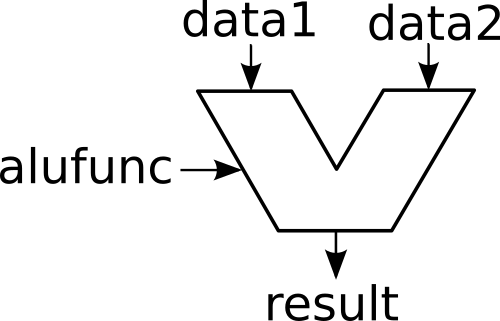
\includegraphics[scale=1]{assets/ALU_block.png}
    \caption{Blokové shéma ALU (převzato z \cite{wiki_ALU})}
    \label{fig:ALU}
\end{figure}

\subsection{Testování aritmetiko logické jednotky}
V souboru \verb|tb_ALU_control.vhd| je obsažná simulace testující funkci ALU a jejího řízení.

\begin{figure}[h]
    \centering
    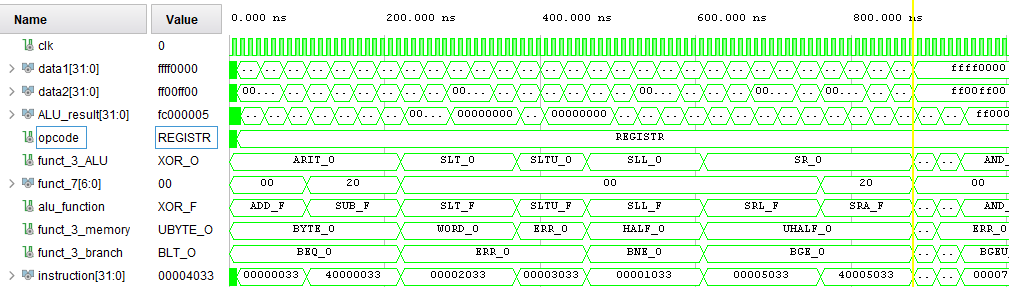
\includegraphics[width=\textwidth]{assets/ALU_simulation.png}
    \caption{Úspěšná simulace ALU}
    \label{img:ALU_simulace}
\end{figure}

\newpage

V simulaci se testují operace sčítání, odčítání, bitový posun, rotace, porovnání a  operace booleovské algebry.

V obrázku \ref{img:ALU_simulace} je uveden záznam signálů ze simulace v prostředí Vivado. 
Simulace využívá příkazu \verb|assert| pro porovnání očekávané hodnoty a té vypočtené v ALU. Při zaznamenaní neshody se do konzole vypíše chybové hlášení. 

\subsection{Využití prostředků na FPGA}
V přílohách je uvedeno schéma ALU\index{ALU} \ref{appendix:ALU}, tak jak jej vygenerovalo IDE Vivado podle popisu VHDL\index{VHDL} kódu. 

\begin{table}[h]
    \caption{Využití prostředku FPGA pro ALU}
    \label{table:ALU_resources}
    \begin{center}
        \begin{tabular}{|l|c|c|c|}
        \hline
        \textbf{Název} & \textbf{Slice LUTs} & \textbf{F7 Muxes} & \textbf{DSP} \\
        \hline
        ALU & 442 & 26 & 0 \\
        \hline
        \end{tabular}
    \end{center}
\end{table}

Syntéza nepřidělila návrhu žádné DSP\index{DSP}\footnote{DSP - digital signal procesing.} bloky, jelikož pracuje nad kratšími slovy než je 32 bitů. Další z důvodů je že pro sčítání a logické operace její použití není tolik přínosné, jako tomu je například u násobení. Instrukci násobení tento procesor ale neimplementuje.

\section{Čítač instrukcí}
Obvod čítače instrukcí drží hodnotu adresy paměti, kde se nachází aktuální instrukce. Při přechodu na další instrukci se k hodnotě v registru přičte $+4$\footnote{Je to posun o $+32b = +4*8b$, protože paměť je bajtově adresovatelná.}. 
Když se má vykonat skok na instrukci, tak se nepřičítá čtyři, ale dojde k přičtení buď hodnoty \verb|imm|, nebo se do registru uloží výsledek z ALU. Entita je popsána v souboru \verb|PC_driver.vhd|.

Obvod je vybaven detektorem nezarovnaných adres, pokud takový stav nastane, nastaví signál \verb|pc_error <= '1'|. 
Tabulka využití HW prostředků FPGA \ref{table:PC_resources}.

\begin{table}[h]
    \caption{Využití prostředku FPGA pro čítač instrukcí}
    \label{table:PC_resources}
    \begin{center}
        \begin{tabular}{|l|c|c|}
        \hline
        \textbf{Název} & 
        \textbf{Slice LUTs} & 
        \textbf{Slice Registers} \\
        \hline
        čítač instrukcí & 20 & 32 \\
        \hline
        \end{tabular}
    \end{center}
\end{table}

\begin{figure}[h]
    \centering
    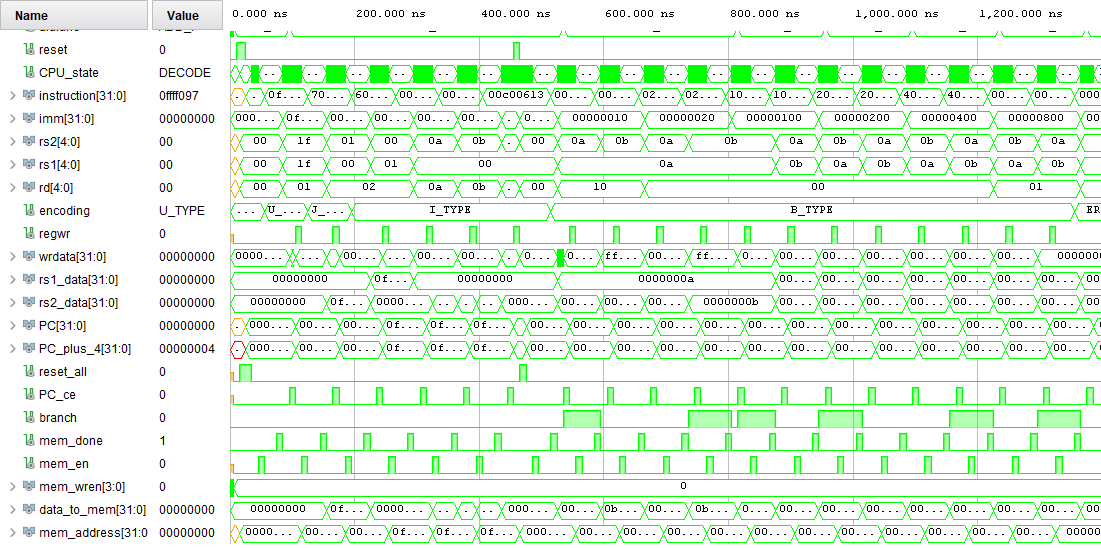
\includegraphics[width=\textwidth]{assets/PC_simulation.png}
    \caption{Úspěšná simulace řízení skoků v programu}
    \label{img:PC_simulace}
\end{figure}

Simulace čítače instrukcí se nachází v souboru \verb|tb_PC_control.vhd|. Povšimněte si v simulaci \ref{img:PC_simulace} jak je signál \verb|branch| nastavován do jedničky v případech, kdy se má skákat v programu.

\section{Paměť}
RAM je řešena jako dvouportová paměť, která je jedním portem připojena přes odvod \verb|memory_wpraper| na datovou sběrnici procesoru RISC-V a druhým portem přes sběrnici AXI do procesoru ARM. Paměť je nakonfigurovaná s latencí dva takty a je popsána v souboru \verb|bram_xpm_wrapper.vhd|. 

Součástí adresního prostoru paměti RAM jsou také MMAP\footnote{Periferie mapované do paměti.} periferie, ty jsou připojené po společné sběrnici kterou tvoří:
\begin{itemize}
    \item adresa,
    \item data do periferie,
    \item data z periferie,
    \item povolení zápisu do bajtů,
    \item signál data vybavena z paměti.
\end{itemize}

Obvod \verb|memory_wpraper| obaluje každou periferii zvlášť a zajišťuje výběr periferie se kterou procesor právě hovoří. Výběr se provádí na základě rozsahu adres, které se předávají jako generický parametr, pokud je periferie vybrána dává se jí to najevo jedničkou na signálu hodiny povoleny (ce).

Paměť RAM je tvořena právě jednou blokovou pamětí.

\subsection{Nezarovnaný přístup do paměti}
Přístup do paměti je realizován po slovech (32b), ale ISA určuje že paměť musí umožnit přístup na jednotlivé bajty. Podrobnosti najdete v kapitole \ref{kap:Instrukce pro práci s pamětí} na straně \pageref{kap:Instrukce pro práci s pamětí}. 

\begin{table}[h]
    \caption{Zarovnaná data v paměti}
    \label{table:zarovnana pamet}
    \begin{center}
        \begin{tabular}{|c|c|c|c|}
        \hline
        \textbf{Bajt 3} & 
        \textbf{Bajt 2} & 
        \textbf{Bajt 1} & 
        \textbf{Bajt 0}
        \\
        \hline
        \multicolumn{4}{|c|}{} \\
        \hline
        \multicolumn{4}{|c|}{slovo}\\
        \hline
        \multicolumn{4}{|c|}{}\\
        \cline{0-1}
        \multicolumn{2}{|c|}{půl slovo} & \multicolumn{2}{c|}{} \\
        \cline{0-2}
        & \multicolumn{2}{c|}{půl slovo} & \\
        \cline{2-4}
        \multicolumn{2}{|c}{} & \multicolumn{2}{|c|}{půl slovo} \\
        \cline{3-4}
        \multicolumn{4}{|c|}{} \\
        \cline{0-0}
        bajt & \multicolumn{3}{c|}{}
        \\
        \cline{0-1}
        & bajt & \multicolumn{2}{c|}{} \\
        \cline{2-3}
        \multicolumn{2}{|c|}{} & bajt & \\
        \cline{3-4}
        \multicolumn{3}{|c|}{} & bajt \\
        %\cline{4-4}
        %\multicolumn{4}{|c|}{} \\
        \hline
        \end{tabular}
    \end{center}
\end{table}

Tabulka \ref{table:zarovnana pamet} reprezentuje všechny možné pozice validního zarovnání dat, které podporuje má implementace přístupu do paměti. Kontrolu provádí funkce \verb|unaligned_address_check| na základě vybrané \verb|funct_3_memory| (slovo, půlslovo, bajt) a adresy posunutí bajtu. 

Zapisovaní dat se dává paměti najevo nastavením signálu povolující zápis na úrovni jednotlivých bajtů, tím se řeší zápisy menší než celé slovo.

Pokud se zapisuje do paměti s adresou bajtu jinou než 0, musí se data před jejich odesláním patřičně posunout do správné pozice.

Při načítání dat z paměti, která jsou posunuta, je třeba je opět zarovnat vpravo. O potřebné zarovnání se stará funkce \verb|data_from_memory_formater|, která umožňuje doplnění nulami, nebo znaménkové rozšíření. 


\begin{table}[h]
    \caption{Nezarovnaná data v paměti}
    \label{table:nezarovnana pamet}
    \begin{center}
        \begin{tabular}{|p{2cm}p{2cm}p{2cm}p{2cm}|}
        \hline
        \multicolumn{1}{|c|}{\textbf{Bajt 3}} & 
        \multicolumn{1}{c|}{\textbf{Bajt 2}} &
        \multicolumn{1}{c|}{\textbf{Bajt 1}} &
        \multicolumn{1}{c|}{\textbf{Bajt 0}} 
        \\
        \hline
        &&& \\
        \cline{2-4}
        & \multicolumn{3}{|c|}{slovo[31:8]}\\
        \hline
        \multicolumn{1}{|c|}{slovo[7:0]} & \multicolumn{3}{c|}{} \\
        \cline{0-0}
        
        \cline{3-4}
        \multicolumn{2}{|c|}{} & \multicolumn{2}{c|}{slovo[31:16]}\\
        \hline
        \multicolumn{2}{|c|}{slovo[15:0]} & \multicolumn{2}{c|}{}\\
        \cline{0-1}

        \cline{4-4}
        \multicolumn{3}{|c|}{} & \multicolumn{1}{c|}{slovo[31:24]}\\
        \hline
        \multicolumn{3}{|c|}{slovo[23:0]} & \multicolumn{1}{c|}{}\\
        \cline{0-2}
        
        \multicolumn{4}{|c|}{}\\
        \cline{0-0}
        \multicolumn{1}{|c|}{půl slov[15:8]} & \multicolumn{3}{c|}{} \\
        \cline{0-0}
        \cline{4-4}
        \multicolumn{3}{|c|}{} & \multicolumn{1}{c|}{půl slovo[7:0]} \\
        %\cline{4-4}
        %\multicolumn{4}{|c|}{} \\
        \hline
        \end{tabular}
    \end{center}
\end{table}

Tabulka \ref{table:nezarovnana pamet} popisuje nezarovnaný způsob uložení dat v paměti. Adresování takto uložených dat nelze se stávající architekturou realizovat pouze jedním přístupem do paměti, proto tento přístup není povolen a dojde k vyvolání výjimky\footnote{Problém však lze vyřešit softwarově při jejím zachycení.}.


\subsection{Připojení paměti k procesoru} \label{kap:Připojení paměti k procesoru}
První návrh počítal se schématem Harvardské architektury počítače, měl tedy oddělenou paměť pro data a instrukce. Výhoda tohoto řešení byla v tom, že je na implementaci jednodušší a disponuje vyšší teoretickou propustností paměti, protože je možné najednou adresovat jak instrukční, tak datovou paměť.  

S touto architekturou jsem otestoval funkčnost načítání příkazů z paměti na programu Fibonacciho posloupnosti, kód uvedený v příloze \ref{listing:fib_asm}. Vše se zdálo velmi nadějné, ale do budoucna to nebyl vhodný přístup. Mít paměť RAM umístěnou uvnitř procesoru a rozdělenou na část pro program a pro data není praktické, protože nemá unifikovaný přístup (nevede k ní jedna společná externí sběrnice). 

Nabízely se různé řešení:
\begin{itemize}
    \item Vyvést z procesoru dvě oddělené sběrnice. 
    \item Přidat vyrovnávací paměť připojenou na jednu sběrnici vedoucí z procesoru.
    \item Přesunout paměti mimo procesor a spojit je v jednu.
\end{itemize}

\paragraph{}
Dvě sběrnice přidávají do návrhu zbytečnou komplexitu, tak jsem toto řešení zahrnul. 

Obalení obou pamětí za pomoci asociativní pamětí (cache\index{cache}), která by měla oddělený přístup jak pro data, tak instrukce je velmi praktické řešení, ale návrh takové paměti je nad rámec zadání práce. 

\paragraph{}
Proto jsem se v dalším kroku návrh rozhodl přesunout paměť mimo procesor. To mělo umožnit připojení periferii mapovaných do paměti a její snazší přeprogramování přes sběrnici AXI (jejíž připojení implementoval vedoucí mé práce). 

Znamenalo to přejít z Harvardského schématu počítače \ref{kap:Harvardské schéma počítače} na Von Neumanovo \ref{kap:Von Neumanovo schéma počítače}, tedy takové, které má jednotnou datovou a adresní sběrnici pro instrukce i data. Byl to nemalý zásah do návrhu a přinesl několik úskalí. Dekodér instrukcí (kombinační logika) předpokládal, že má instrukci stále k dispozici. To se ale s jednotnou sběrnicí změnilo, měl k dispozici buď načtenou instrukci, nebo data. 

Řešením bylo přesunout řízení paměti na stranu procesoru, tak aby ven komunikoval pouze s jednou pamětí, ale vnitřně poskytoval registry pro uchovávání jak dat, tak i instrukce. 
Došlo tedy k přepracování řídící jednotky tak, že do ní byli přesunuty všechny funkce pro formátování dat \textbf{z} a \textbf{do} paměti. Nyní adresu pro komunikaci při jednotlivých fázích procesoru vybírá řídící jednotka. 
Při načítání instrukcí se na adresu do paměti připojí hodnota registru \verb|pc| a ve fázi zápisu nebo čtení dat zase výsledek z ALU. 
Řídíc jednotka pak setrvá v dané fázi než paměť pošle signál data vybavena. 

\paragraph{}
Výsledkem této změny návrhu bylo zpomalení práce fází procesoru, které manipulují s pamětí (načti instrukci a zapiš do paměti), o jeden takt (než se data vybaví a propíší do příslušného registru v řídící jednotce). 

\subsection{Simulace přístupu do paměti}
Simulace \verb|tb_memory_control.vhd| ověřuje čtení a zápis do paměti. Kontroluje zda nezarovnaný přístup vyvolává výjimku. Proto si můžete všimnout, že se v simulaci \ref{img:MEM_simulace} několik aktivuje signál \verb|reset_all|, který resetuje celý procesor včetně hlášení o výjimkách. 

\begin{figure}[h]
    \centering
    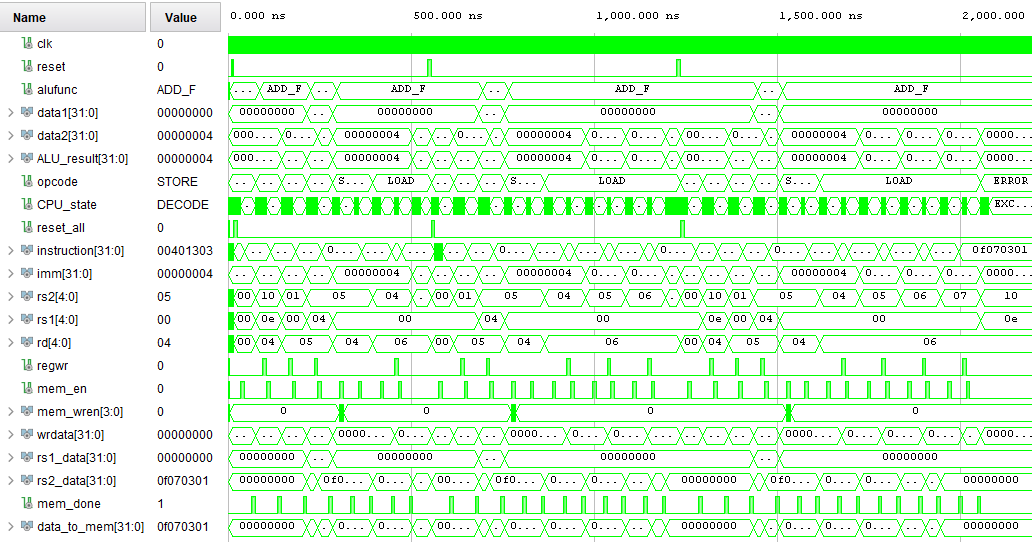
\includegraphics[width=\textwidth]{assets/MEM_simulation.png}
    \caption{Úspěšná simulace přístupu do paměti}
    \label{img:MEM_simulace}
\end{figure}

\subsection{Periferie mapované do paměti}
RISC-V nemá žádné instrukce pro přímou komunikací s vnějšími periferiemi. Pro jejich ovládání se využívá přístupu zařízeních mapovaných do paměti. Na příslušném rozsahu adres jsou místo paměti RAM\index{RAM} připojeny například GPIO I/O registry či frame buffer displeje, nebo jiné periferie. 

V mém návrhu procesoru se využívá periferií LED a přepínačů. Při nahrání hodnoty 0 na příslušnou pozici v rozsahu adres \textbf{směru} se pin periferie na daném bitu nastaví jako výstupní. Při nahrání hodnoty 1 se nastaví jako vstupní. 

V paměti jsou reprezentovány jako 4x32b paměti, kde:
\begin{itemize}
    \item první 4B (adresa+0) jsou směr (direction: in/out) (nastavení vstupu/výstupu periferie), 
    \item další 4B (adresa+4) slouží pro zápis do periferie,
    \item následné 4B(adresa+8) slouží pro vyčítání hodnot z periferie,
    \item poslední 4B (adresa+12) nejsou obsazeny a jsou zde pouze pro zarovnání paměti na násobky dvou.
\end{itemize}

Na periferie lze přistupovat stejně jako do pole, ukázka kódu \ref{listing:asm_switch_to_led} který nastaví LEDky jako výstupní, přepínače jako vstupní a pak vezme hodnotu z přepínačů a nastaví je na LEDky.

\begin{listing}[h]
    \begin{minted}{gas}
# LED addresses (LED_ADDRESS -> RAM_SIZE)
li t3, 4096   
# LED directions, 32 output pins
sw zero, 0(t3) 
# LED values OFF
sw zero, 4(t3) 

# SWITCH addresses (SWITCH_ADDRESS -> RAM_SIZE + LED_SIZE)
# 4096 + 16
addi t4, t3, 16
# SWITCH directions
lui t5, 0xFFFFF
ori t5, t5, -1
sw t5, 0(t4)

# nacteni hodnoty z prepinace
lw s0, 8(t4)
# zapis do led
sw s0, 4(t3)
    \end{minted}
    \caption{Demonstrační kód pro zápis z přepínačů do LED}
    \label{listing:asm_switch_to_led}
\end{listing}

\section{Řídící jednotka} \label{kap:cu}
Zdaleka nejsložitější částí procesoru pro návrh je řídící jednotka. Právě v ní se rozhoduje co bude která část procesoru v daný okamžik vykonávat. 

V průběhu navrhování procesoru prošla řídící jednotka několika různými verzemi. Došlo například k přesunu dekodéru instrukcí do jejích útrob, stejně jako obvodů pro řízení paměti \ref{kap:Připojení paměti k procesoru} a primitivní správy výjimek. 

Řídící jednotka také vyhodnocuje kdy došlo ke skoku v programu.  

\begin{figure}[h]
	\centering
	\begin{tikzpicture}[node distance=2.5cm, every node/.style={draw, minimum width=2cm, minimum height=1cm}]
	
		\node (fetch) {Fetch};
		\node (decode) [right of=fetch] {Decode};
		\node (execute) [right of=decode] {Execute};
		\node (memory) [right of=execute] {Memory};
		\node (writeback) [right of=memory] {Writeback};
		
		\draw[->] (fetch) -- (decode);
		\draw[->] (decode) -- (execute);
		\draw[->] (execute) -- (memory);
		\draw[->] (memory) -- (writeback);
		
	\end{tikzpicture}
	
	\caption{Fáze procesoru}
	\label{fig:cpu_stages}
\end{figure}

Procesor je navržen s ohledem na zřetězené zpracování instrukcí, symbolicky naznačené v diagramu \ref{fig:cpu_stages}. Zatím jej však nepodporuje. V bodovém seznamu je uvedeno pět klasických fází zřetězeného vykonávání procesorů architektury RISC-V:
\begin{itemize}
    \item \textbf{Fetch} - načtení instrukce,
    \item \textbf{Decode} - dekódování instrukce,
    \item \textbf{Execute} - vykonání,
    \item \textbf{Memory} - paměť,
    \item \textbf{Writeback} - zápis do registru.
\end{itemize}

Řídící jednotka je navržena jako stavový automat. Jde o modifikovaný Mealyho automat, jehož všechny výstupy jsou vyvedeny přes registr. Automat je popsán vývojovým diagramem na obrázku \ref{fig:cpu_stages}.

\begin{figure}[h]
    \centering
    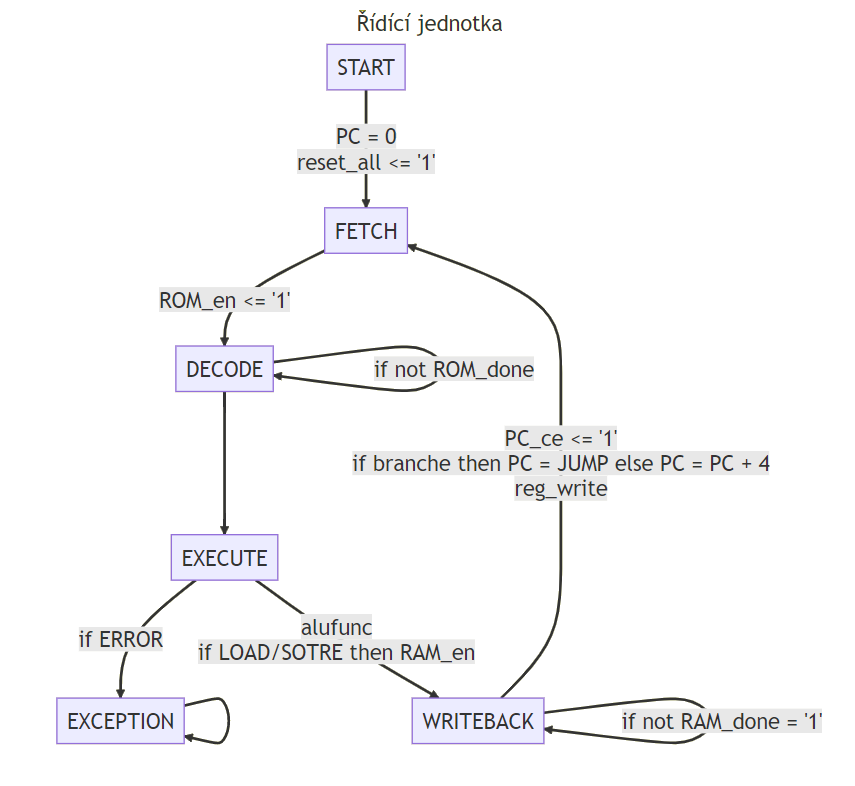
\includegraphics[scale=0.45]{assets/Řídící jednotka.png}
    \caption{Vývojový diagram řídící jednotky}
    \label{fig:control_cycle}
\end{figure}

Fáze mého stavového automatu se skládají z: 
\argument{START}, 
\argument{FETCH}, 
\argument{DECODE}, 
\argument{EXECUTE}, 
\argument{MEMORY}, 
\argument{WRITEBACK}, 
\argument{HALT}, 
\argument{EXCEPTION}.

Při restartování procesoru se nastaví fáze stavového automatu na \argument{START}. Když nastane vyjímka tak automat skočí na \argument{EXCEPTION} a následně přejde do stavu \argument{HALT}, ve kterém setrvá až do restartování. 

\begin{table}[h]
    \caption{Využití prostředku FPGA pro řídící jednotku}
    \label{table:CU_resources}
    \begin{center}
        \begin{tabular}{|l|c|c|c|}
        \hline
        \textbf{Název} & 
        \textbf{Slice LUTs} & 
        \textbf{Slice Registers} & 
        \textbf{F7 Muxes} \\
        \hline
        řídící jednotka & 857 & 113 & 7 \\
        \hline
        \end{tabular}
    \end{center}
\end{table}

V tabulce \ref{table:CU_resources} jsou uvedeny HW požadavky na FPGA.

\paragraph{}
Ač můj návrh architektury staví na instrukční sadě RISC 
kapitola \ref{kap:RISC}, tak jeho řídící jednotka vykazuje známky přístupu které jsou běžné pro architekturu CISC kapitola \ref{kap:CISC}. Umožňuje vykonání instrukcí proměněného počtu taktů a to jmenovitě při práci s pamětí. Řídící jednotka při načítání a ukládání dat čeká na signál data vybavena. Tímto způsobem je ošetřena vícetaktová vybavovací doba blokové paměti (2 takty) ze které je nakonfigurovaná RAM\index{RAM} pomocí makra XPM.  
Výhoda tohoto přístupu se naplno projeví až v budoucnu při implementování asociativní paměti (cache\index{cache}) procesoru. Při nalezení (hit) se budou instrukce načítat rychleji (jeden takt) a při případném nenalezení (miss) se vykonávání automaticky pozastaví, protože řídící jednotka bude čekat na signál vybavení dat z paměti RAM.

\newpage
\section{Jádro procesoru RISC-V a RAM}
V jádru procesoru se propojují jednotlivé části návrhu. Jsou v něm také definovány multiplexery pro výběr zdroje pro zápis do registru a argumentů ALU. K jádru procesoru je ještě připojená paměť a MMAP periferie. 

\begin{table}[h]
    \caption{Využití prostředku FPGA pro jádro procesoru RISC-V}
    \label{table:RISC-V_core_resources}
    \begin{center}
        \begin{tabular}{|l|c|c|c|c|}
        \hline
        \textbf{Název} & 
        \textbf{Slice LUTs} & 
        \textbf{Slice Registers} & 
        \textbf{F7 Muxes} & 
        \textbf{F8 Muxes} \\
        \hline
        jádro procesoru & 1624 & 1137 & 263 & 70 \\
        \hline
        \end{tabular}
    \end{center}
\end{table}

HW požadavky toho návrhu jsou uvedeny v tabulce \ref{table:RISC-V_core_resources}.


\section{Vlastní IP jádro}
Aby bylo možné nahlížet do operační paměti procesoru je k ní souboru \verb|computer_wrapper.vhd| ještě připojena AXI sběrnice, která ARM procesoru umožňuje přístup do paměti. Jsou zde také napojené vstupní a výstupní periferie (LED, přepínače a GPIO) na piny FPGA.

\begin{table}[h]
    \caption{Využití prostředku FPGA pro IP jádro}
    \label{table:IP_core_resources}
    \begin{center}
        \begin{tabular}{|l|p{1.5cm}|c|c|c|p{1.5cm}|c|}
        \hline
        \textbf{Název} & 
        \textbf{Slice LUTs} & 
        \textbf{Slice Registers} & 
        \textbf{F7 Muxes} & 
        \textbf{F8 Muxes} & 
        \textbf{Block RAM} & 
        \textbf{I/0} \\
        \hline
        IP jádro & 1936 & 1783 & 263 & 70 & 1 & 178 \\
        \hline
        IP jádro & 3,6\% & 1,7\% & 1\% & 0,5\% & 0.7\% & 90\% \\
        \hline
        Zynq7020 & 53200 & 106400 & 26600 & 13300 & 140 & 200\\
        \hline
        \end{tabular}
    \end{center}
\end{table}

Návrh procesoru využívá přibližně 3,7\% LUTů, 1,7\% registrů. Informace o využitých I/O je zavádějící protože naprostá většina z nich slouží pro implementaci AXI sběrnice, pokud by design RISC-V uCPU tvořil výsledný návrh, většina z I/O by nebyla připojená na piny FPGA. Takže ve srovnání s prostředky FPGA je můj návrh velmi malý. 



\chapter{Programy}\label{kap:Programy}
Tato práce se kromě návrhu architektury jádra procesoru RISC-V v jazyce VHDL\index{VHDL} zabývala i vývojem testovacích programů a nástrojů potřebných pro jejich nahrání do paměti.

Pro otestování funkčnosti jsem napsal několik programů v jazyce symbolických adres. Lze je rozdělit do dvou skupin dle určení:
\begin{itemize}
    \item pro použití v simulaci,
    \item pro syntetizovaný procesor na desce FPGA\index{FPGA}.
\end{itemize}

\section{Programování procesorů RISC-V}
V následujících kapitolách se nejprve lehce seznámíme s psaním programů v jazyce assembly pro procesory RISC-V.

\subsection{Pseudoinstrukce}
Pseudoinstrukce slouží pro větší abstrakci při programování v jazyce symbolických adres (assembly). Umožňují psát program v instrukcích, které procesor sice přímo nepodporuje, ale jejich vykonání je možné syntetizovat pomocí již existujících instrukcí (obrázek \ref{img:RISC-V_insturctions}) a to buď zaměněním pořadí argumentů, či případně vynulováním jednoho z nich, viz tabulka \ref{table:pseudoinstructions}. 

Například instrukce MV (přesun obsah registru) jde syntetizovat jako \verb|ADDI rd, ra1, 0|. V tabulce \ref{table:pseudoinstructions} je přehled dalších pseudoinstrukcí. 

\newpage

\begin{table}[h]
    \caption{RISC-V pseudoinstrukce (převzato z \cite{Harris2021})}
    \label{table:pseudoinstructions}
    \begin{center}
    \scalebox{0.8}{
        \begin{tabular}{|llll|llll|l|}
        \hline
        \multicolumn{4}{|c|}{\textbf{Pseudoinstrukce}} &
        \multicolumn{4}{c|}{\textbf{RISC-V instrukce}} &
        \multicolumn{1}{c|}{\textbf{Popis}}
        \\
        \hline
        nop &&& & 
        addi & x0, & x0, & 0 &
        nedělej nic
        \\
        \hline
        li & rd, & imm$_{11:0}$ & &
        addi & rd, & x0, & imm$_{11:0}$ &
        načti 12-bitovou konstantu 
        \\
        \hline
        li & rd, & imm$_{31:0}$ & &
        lui & rd, & imm$_{31:12}$ & &
        načti 32-bitovou konstantu
        \\
        &&&& 
        addi & rd, & rd, & imm$_{11:0}$ &
        \\
        \hline
        mv &rd, &rs1 &&
        addi &rd, &rs1, &0&
        přesun
        \\
        \hline
        not & rd, & rs1 && 
        xori & rd, & rs1, & $-1$ & 
        jedničkový doplněk
        \\
        \hline
        neg & rd, & rs1 & &
        sub & rd, & x0, & rs1 & 
        dvojkový doplněk
        \\
        \hline
        seqz & rd, & rs1 &&
        sltiu & rd, & rs1, & 1 & 
        nastav když = 0
        \\
        \hline
        snez & rd, & rs1 &&
        sltu & rd, & x0, & rs1& 
        nastav když $\neq 0$
        \\
        \hline
        sltz &rd, &rs1 & &
        slt &rd, &rs1, &x0 & 
        nastav když $< 0$
        \\
        \hline
        sgtz &rd, &rs1 &&
        slt &rd, &x0, &rs1& 
        nastav když $> 0$
        \\
        \hline
        beqz &rs1, &label &&  
        beq &rs1, &x0, &label& 
        skoč když $= 0$
        \\
        \hline
        bnez & rs1, &label &&
        bne &rs1, &x0,& label& 
        skoč když $\neq 0$
        \\
        \hline
        blez &rs1,& label &&  
        bge &x0, &rs1,& label& 
        skoč když $\leq 0$
        \\
        \hline
        bgez &rs1, &label &&
        bge &rs1, &x0, &label & 
        skoč když $\ge 0$        
        \\
        \hline
        bltz &rs1, &label &&
        blt &rs1, &x0,& label & 
        skoč když $< 0$
        \\
        \hline
        bgtz &rs1, &label &&  
        blt &x0, &rs1, &label & 
        skoč když $> 0$
        \\
        \hline
        ble &rs1, &rs2, &label &  
        bge &rs2, &rs1, &label & 
        skoč když $\le$
        \\
        \hline
        bgt &rs1, &rs2, &label &  
        blt &rs2, &rs1, &label & 
        skoč když $>$
        \\
        \hline
        bleu &rs1, &rs2, &label &  
        bgeu &rs2, &rs1, &label & 
        skoč když $\le$ (ne znaménkově)
        \\
        \hline
        bgtu &rs1, &rs2, &label &  
        bltu &rs2, &rs1, &offset & 
        skoč když $>$ (ne znaménkově)
        \\
        \hline
        j & label &&&  
        jal &x0, &label & &
        skoč        
        \\
        \hline
        jal &label &&&  
        jal &ra, &label & &
        skoč a ulož adresu
        \\
        \hline
        jr &rs1 &&&
        jalr &x0, &rs1, &0 & 
        skoč na registr
        \\
        \hline
        jalr &rs1 &&&  
        jalr &ra, &rs1,& 0 & 
        skoč na registr a ulož adresu
        \\
        \hline
        ret & &&&
        jalr &x0, &ra,& 0 & 
        návrat z funkce
        \\
        \hline
        call &label &&&  
        jal &ra, &label && 
        zavolání funkce
        \\
        \hline
        \end{tabular}
    }
    \end{center}
\end{table}

\subsection{Zápis instrukcí v jazyce symbolických adres}
Instrukce se skládá z názvu instrukce a argumentů. Argumenty jsou odděleny čárkou a mohou být v závorce. Argumenty mohou být indexy registrů, konstanty, nebo adresy do paměti. 

\begin{listing}[h]
    \begin{minted}{gas}
inst rd, rs1, rs2
inst rd, rs1, imm
jmp rd, imm
    \end{minted}
    \caption{Zápis instrukcí v jazyce symbolických adres}
    \label{listing:asm_instructions}
\end{listing}

Jak je vyobrazeno v kódu \ref{listing:asm_instructions}, pořadí argumentů je následující: cílový registr, první zdrojový registr, druhý zdrojový registr. Pokud je v instrukci pouze jeden registr, tak je to cílový registr. 

\subsection{Inicializace procesoru}
Procesor je potřeba před spuštěním vyresetovat. To smaže obsah všech registrů a shodí všechny případné výjimky. Pokud náš program pracuje se zásobníkem, tak je potřeba nejprve provést inicializaci registru \verb|x2| (\verb|sp|\index{sp} - stack pointeru) na horní hranici rozsahu paměti RAM\index{RAM}, příklad kódu \ref{listing:asm_init}. Operační paměť má nastavenou syntetizovanou velikost 4kB (4096 bajtů).

\begin{listing}[h]
    \begin{minted}[linenos]{gas}
# MEM(0:4092)
# WORD_SIZE = 4
li sp, 4096
addi sp, sp, -4
    \end{minted}
    \caption{Inicializace ukazatele na zásobník}
    \label{listing:asm_init}
\end{listing}

\subsection{Volání funkcí}
Volání funkcí v jazyce symbolických adres je znázorněno v kódu \ref{listing:asm_func}. Symbol \verb|func| je zde použit pro název funkce a používá se jako reference na adresu následující instrukce.

\begin{listing}[h]
    \begin{minted}[linenos]{gas}
func:
    # tělo funkce
    ret

jal ra, func
    \end{minted}
    \caption{Zápis funkcí v jazyce symbolických adres}
    \label{listing:asm_func}
\end{listing}

Příkaz \verb|jal| (jump and link) provede skok na adresu funkce a uloží si do registru \verb|ra|\index{ra} adresu následující instrukce. Tento registr se používá pro návrat z funkce. Příkaz \verb|ret| (return) provede skok na adresu uloženou v registru \verb|ra|\index{ra}. Jako registry argumentů se standardně používají registry \verb|a0| až \verb|a7|. Pro uložení návratových hodnot slouží registry \verb|a0| a \verb|a1|, viz \ref{table:registers}.

\subsection{Začínáme ve funkci main}
Je možné, že náš program po inicializaci registrů obsahuje deklarace funkcí, které chceme při spuštění přeskočit. Skok na hlavní program vykoná instrukce: \verb|j main|. Příkaz \verb|j| (jump) provede skok na adresu funkce (main). 

\newpage

\subsection{Program v Assembly}
Takto by mohl vypadat demonstrační program \ref{listing:asm_program}, který běží v nekonečné smyčce. Funkce \verb|return_arg| vrací svůj argument. Program main, volá funkci \verb|return_arg| a ta svůj argument \verb|a0| ukládá jako návratovou hodnotu do registru \verb|a1|. Pokud je návratová hodnota různá od nuly, tak se program vrátí na začátek smyčky \verb|loop|. Pokud je návratová hodnota nula, tak se program ukončí vyvoláním výjimky instrukcí \argumentindex{ECALL}.

\begin{listing}[h]
    \begin{minted}[linenos]{gas}
.text
.globl main

# inicializace ukazatele na zasobnik
li sp, 4096         # MEM(0:4092)
addi sp, sp, -4     # WORD_SIZE = 4

j main              # skok na smycku hlavni funkce

# Funkce: return argumet
# Argumenty:
#  a0 - argument
#  a1 - navratova hodnota
return_arg:
    mv a1, a0       # a1 = a0
    li a0, 0        # a0 = 0
    ret

main:
    addi a0, x0, 1  # a0 = 1

    loop:
        jal ra, return_arg  # a1 = return_arg(a0)
        addi a0, a1, 0      # a0 = a1
        bne a1, x0, loop    # if a1 is True goto loop
    ecall
    \end{minted}
    \caption{Ukázka programu v jazyce symbolických adres}
    \label{listing:asm_program}
\end{listing}

Direktiva \verb|.text| říká, že následující příkazy jsou instrukce programu a budou uložena v sekci paměti \textbf{text}, blíže v kapitole \ref{kap:Text} na straně \pageref{kap:Text}. Direktiva \verb|.globl| nastavuje následující symbol jako globální, ten pak může být použit i v jiných souborech. V tomto případě je to symbol \verb|main|.

\section{Kompilace zdrojových kódů}
Program v jazyce C není zas tak jednoduché přeložit do binárního kódu spustitelného na architektuře RISC-V32I. Při překladu na počítači s procesorem architektury Intel/AMDx64 je potřeba využít takzvaného křížového překladu\footnote{Program je kompilovaný pro jinou rodinu procesoru, než do které patří procesor, který překlad provádí.}. Problém je však v tom, že existují běžné překladače pro RISC-V64G\footnote{G je zkratka pro rozšíření IMAFDZicsr\_Zifencei.}, tento kód na mém procesoru nelze spustit. 

Při překladu z jazyka symbolických adres lze využít běžného RISC-V překladače, pokud však jsou instrukce programu pečlivě voleny tak, aby obsahovaly pouze instrukce z ISA RISC-V32I.

\subsection{Vlastní překlad překladače}
Je možné si přeložit překladač z jazyka C a Assembly pro RISC-V32I. Na GitHubu je hostován organizací RISC-V Collaboration projekt riscv-gnu-toolchain, odkaz \href{https://github.com/riscv-collab/riscv-gnu-toolchain}{\emph{zde}}. Který obsahuje nástroje pro sestavené křížového překladače pro RISC-V \cite{github_GNU_compiler}.

\begin{quote}[Urban dictionary \cite{urbandictionary_Ubuntu}]{Ubuntu}
Ubuntu je pradávné africké slovo nesoucí význam: „Neumím nakonfigurovat Debian“.
\end{quote}

Překladač GNU jsem úspěšně přeložil na stroji s operačním systémem Ubuntu Linux. Šlo o časově velice náročnou operaci (několik hodin). Prostředí IDE Vivado\index{Vivado} mám však nainstalované na počítači s operačním systémem Windows. Nabízelo se překladač používat pod WSL, ale já jsem zvolil snazší variantu a to používat překladač dostupný online. Pokud bych měl v budoucnu překládat delší zdrojové kódy jazyka symbolických adres, případně C, jistě bych se vydal cestou přes WSL. 

\subsection{Překlad z jazyka symbolických adres v online překladači}
Mnohem snazší je pro začátek použít online překladač z jazyka symbolických adres na kód v šestnáctkové (hexa) 
 pro procesory RISC-V: 
\href{https://riscvasm.lucasteske.dev/#}{\emph{riscvasm.lucasteske.dev}}.
Jde o velmi jednoduchý překladač na ovládání. Po vložení zdrojového kódu stačí zmáčknout tlačítko "BUILD" a kód se přeloží do hexa souboru. Webová stránka poskytuje i disassembly výstup pro zpětný přepis na instrukce, který obsahuje již i čísla adres v paměti vizualizující jednotlivé skoky na návěští (symboly).

\newpage

\section{Generování konfiguračních souborů pro nahrání programu do paměti} \label{kap:generování souborů s programem}
Přeložený program jde ukládat do několika různých formátů:
\begin{itemize}
    \item \textbf{CEO} - slouží pro konfigurátor IP jader (ten se v poslední návrhu procesoru již nevyužívá, nahradil jej popis paměti přímo v XPM),
    \item \textbf{MEM} - je formát pro blokové paměti. Programy z tohoto formátu načítá simulace.
    \item \textbf{RAW} - slouží k ukládání na SD kartu pro desku ZedBoard.
\end{itemize}
Pro usnadnění práce s těmito soubory byl vytvořen python script \verb|RISC-V/programs/vivado_datafile_generator.py| ten umožňuje přepis hex-dump souboru do formátu \verb|.coe, .mem, .raw|. Ukázka výpisu přepínače \verb|--help| pro zmíněný program \ref{listing:python_program}.

\begin{listing}[h]
    \begin{minted}{bash}
python.exe .\vivado_datafile_generator.py --help
usage: vivado_datafile_generator.py [-h] -i INPUT [-o OUTPUT] 
                                    [-r RADIX] [-f FORMAT]    

Aplication for generating COE, RAW and MEM files. For VHDL ROM
initialization. Specific types: 
- COE file is used for Xilinx Vivado block ram IP core. 
- MEM file is used for block ram. 
- RAW file is used for loading program into FPGA memory from SD card.

options:
  -h, --help            show this help message and exit       
  -i INPUT, --input INPUT
                        input file
  -o OUTPUT, --output OUTPUT
                        output file
  -r RADIX, --radix RADIX
                        radix
  -f FORMAT, --format FORMAT
                        file format
    \end{minted}
    \caption{Python skript pro generování Xilinx souborů s programem}
    \label{listing:python_program}
\end{listing}

Příklad použití, pro vygenerování nového souboru \verb|.mem| s obsahem paměti ze souboru \verb|sum.txt| zadejte příkaz:

\paragraph{}
\verb|python3 vivado_datafile_generator.py -i sum.txt -o program.mem|

\section{Demo programy pro otestování RISC-V procesoru v simulaci}

\subsection{Test aritmetiky}
Pro základní test aritmetiky byl zvolen program výpočtu sumy. Vzniklo několik jeho variant. První varianta testuje pouze základní aritmetické operace a cyklus for. Druhá varianta testuje i volání funkce.

\begin{figure}[h]
    \centering
    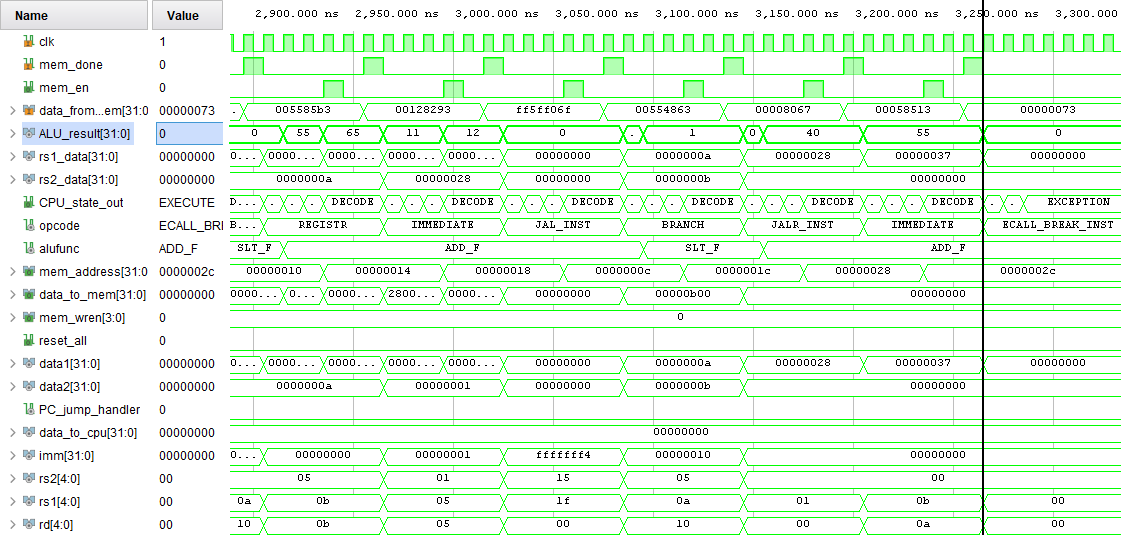
\includegraphics[width=\textwidth]{assets/Program_sum(10).png}
    \caption{Úspěšná simulace se spuštěním programu sum(10)}
    \label{img:sum_simulace}
\end{figure}

V simulaci \ref{img:sum_simulace} je spuštěn program sečti posloupnost čísel od $1$ do $10$.
Všimněte si že výsledek je v signálu \verb|ALU_result| má hodnotu $55$.

\subsection{Test paměti}
Program testující práci s pamětí, které bude později využita při ukládání proměnných na zásobník a jejich čtení, nebo při komunikaci se zařízeními mapovanými do paměti. Cyklus for postupně ukládá do paměti data, následně je čte a ověřuje zda jsou shodná. Začne na čísle 0 a postupně inkrementuje až do velikosti paměti. S hodnotou proměnné se posouvá i adresa, na kterou se má data uložit. Pokud se někde vyskytne chyba, program se ukončí. Simulace je uvedena n obrázku \ref{img:mem_test_simulace}.

\begin{figure}[h]
    \centering
    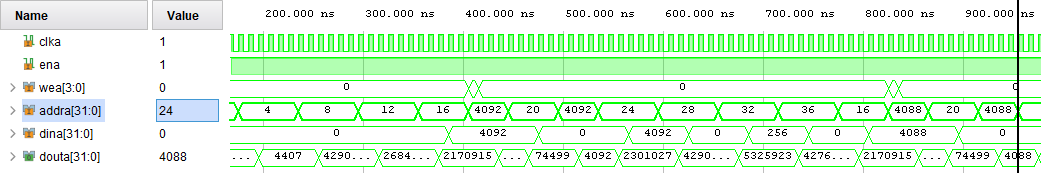
\includegraphics[width=\textwidth]{assets/Program_mem_test.png}
    \caption{Úspěšná simulace se spuštěním programu testu paměti}
    \label{img:mem_test_simulace}
\end{figure}

\subsection{Fibonacci}
Algoritmus Fibonacciho posloupnosti byl zvolen protože pro výpočet nepotřebuje operace násobení a dělení. Nejdříve byla využita jeho sekvenční verze, která využívá cyklus for, pro otestování základní funkčnosti. Následně byla využita rekurzivní verze, která využívá zásobník. Program v jazyce C je uveden v příloze \ref{listing:fib_c}, stejně tak i ten v jazyce symbolických adres příloha \ref{listing:fib_asm}. 

\begin{equation}
F(n) = 
\begin{cases}
0, & \text{pro } n = 0; \\
1, & \text{pro } n = 1; \\
F(n−1)+F(n−2) & \text{jinak.}
\end{cases}
\end{equation}
%\caption{Předpis Fibonacciho posloupnosti}
%\label{equations:fib}

\begin{figure}[h]
    \centering
    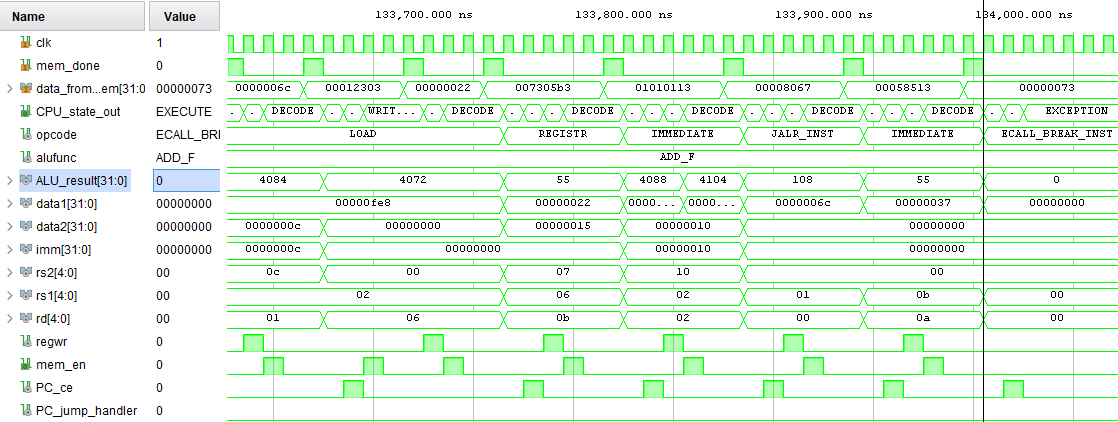
\includegraphics[width=\textwidth]{assets/Program_fib(10).png}
    \caption{Úspěšná simulace se spuštěním programu fib(10)}
    \label{img:fib_simulace}
\end{figure}

Při syntéze RAM o velikosti 4kB se na stack se vejde $256$ rámců ($256 * 16B = 4kB$). V každém rámci jsou 4B pro uložení adresy návratu a $12$B pro uložení argumentů. Tedy maximálně $256$ volání rekurze. Při volání výpočtu $fib(10)$ je potřeba zavolat funkci $177$ a to se s jistotou do paměti RAM vejde.

Ze simulace \ref{img:fib_simulace} je patrné, že po uplynutí času $134 us$ se procesor dopočítá k hodnotě $fib(10) = 55$, což je očekávaný výsledek. 

\subsection{Nahraní nového programu do simulace}
Simulace (test bench) \verb|tb_run_program.vhd| spouští program uložený do souboru: \verb|program.mem|. Pro spuštěné nového programu je potřeba vygenerovaný soubor ve formátu \verb|.mem| přesunout do adresáře \verb|./RISC-V.srcs/sources_1/new/| a restartovat simulaci.

\section{Demo programy pro RISC-V procesor na desce ZedBoard}
Procesor je také napojen na vnější svět pomocí zařízení mapovaných do paměti. Je připojený na přepínače a ledky. Ledky jsou mapované na adresu 4096 a mají rozsah 128b. Přepínače na adresu 4112. Přepínače jsou nastaveny jako vstupní a ledky jako výstupní piny. 

Pro otestování vývojové desky byl napsán program \verb|switch_to_LED|, který běží v nekonečné smyčce a zrcadlí stav přepínačů na ledkách.

Funkčnost syntetizované architektury se tímto jednoduchým programem podařila úspěšně ověřit.

\subsection{Nahrání programu do paměti}
Vývojová deska je postavené kolem SoC Xilinx Zynq-7000, který má v sobě jak FPGA\index{FPGA}, tak i ARM procesor. Pro něj vedoucí mé práce vytvořil program v jazyce C. Program hledá na SD kartě soubor \verb|program.raw|. Když soubor s příponou \verb|.raw| úspěšně nalezne, tak jeho obsah nahraje do paměti RAM procesoru RISC-V který je syntetizovaný v části čipu s FPGA. 

Teto program se následně postará i o řízení mého procesoru. Povoluje mu signál hodin (jeden takt, nebo více) a pokud je k ARMu připojen váš počítač po sériové lince, umožní i výpis do konzole v jaké fázi se procesor nachází. 

\paragraph{}
Jak vytvořit soubor s příponou \verb|.raw| pro nahrání programu je podrobněji popsáno v kapitole \ref{kap:generování souborů s programem}.

Vygenerovaný soubor nakopírujte na SD kartu a zasuňte jí do vývojové desky ZedBoard. Desku restartujte. Když spustíte aplikaci pro nahrávání programu na procesoru ARM přes IDE Vitis\index{Vitis}, tak se provede jeho zavedení do paměti procesoru RISC-V a ten bude uveden v činnost. 

\chapter{Závěr}

V bakalářské práci jsem se seznámil se specifikací ISA RISC-V. Podle ní jsem navrhl procesorové jádro v základní 32bitové verzi, které pracuje v neprivilegovaném režimu. Můj procesor umožňuje výpočty s celými čísly a je bez jakéhokoliv rozšíření. Navržené jádro jsem propojil s operační paměti a vstupními a výstupními periferiemi. 

V simulacích jsem postupně úspěšně otestoval základní vlastnosti tohoto procesoru, jako jsou aritmetickologické operace, přístup do paměti nebo podmíněné skoky v programu. 

Podařilo se mi syntetizovaný procesor nahrát do FPGA\index{FPGA} řady Xilinx Zynq-7000. Nakonec jsem napsal program v jazyce symbolických adres pro zobrazení stavu přepínačů na LED diodách. Tento program se na mém procesoru úspěšně spustil.

\paragraph{}
Nejpřímočařejším rozšířením mého procesoru by bylo přidání některého z rozšíření které popisuje specifikace ISA RISC-V, jako je například podpora násobní a dělení, nebo výpočtů nad čísly s pohyblivou řádovou čárkou. 

Do budoucna se nabízí procesor také rozšířit o zřetězené zpracovávání instrukcí. Při návrhu jsem se snažil postupovat tak, aby implementace tohoto rozšíření byla co nejednodušší. 

Dalším způsobem navýšení výkonu mého procesoru by mohlo být jeho doplnění o asociativní paměť.

Pokud nastane výjimka při vykonávání programu, tak se můj procesor zastaví. Vhodným rozšířením by tak z tohoto pohledu bylo navrhnout obsluhu výjimek, třeba i s programovou částí řešící limitace základní ISA RISC-V32I jako je například chybějící instrukce násobení nebo podpora práce s nezarovnanou pamětí.

Můj procesor sice nedisponuje nikterak vysokým výkonem, ale jeho výhodou jsou malé rozměry (zabere méně než 4\% LUTů) na FPGA řady Xilinx Zynq-7000. Při rozšíření návrhu o sérii čítačů, a podporu přerušení by mohl sloužit jako mikroprocesor pro ovládání jiných návrhů na FPGA, které potřebují procesorové řízení. 

\paragraph{}
Zajímavé by bylo také prozkoumat tu možnost kdy by se z mého návrhu nechal pouze balíček implementující specifikaci RISC-V a návrh procesoru by se přepsal do čistě behaviorální podoby, která by stavěla na funkcích z balíčku, jejichž funkčnost je již otestovaná. 


\appendix

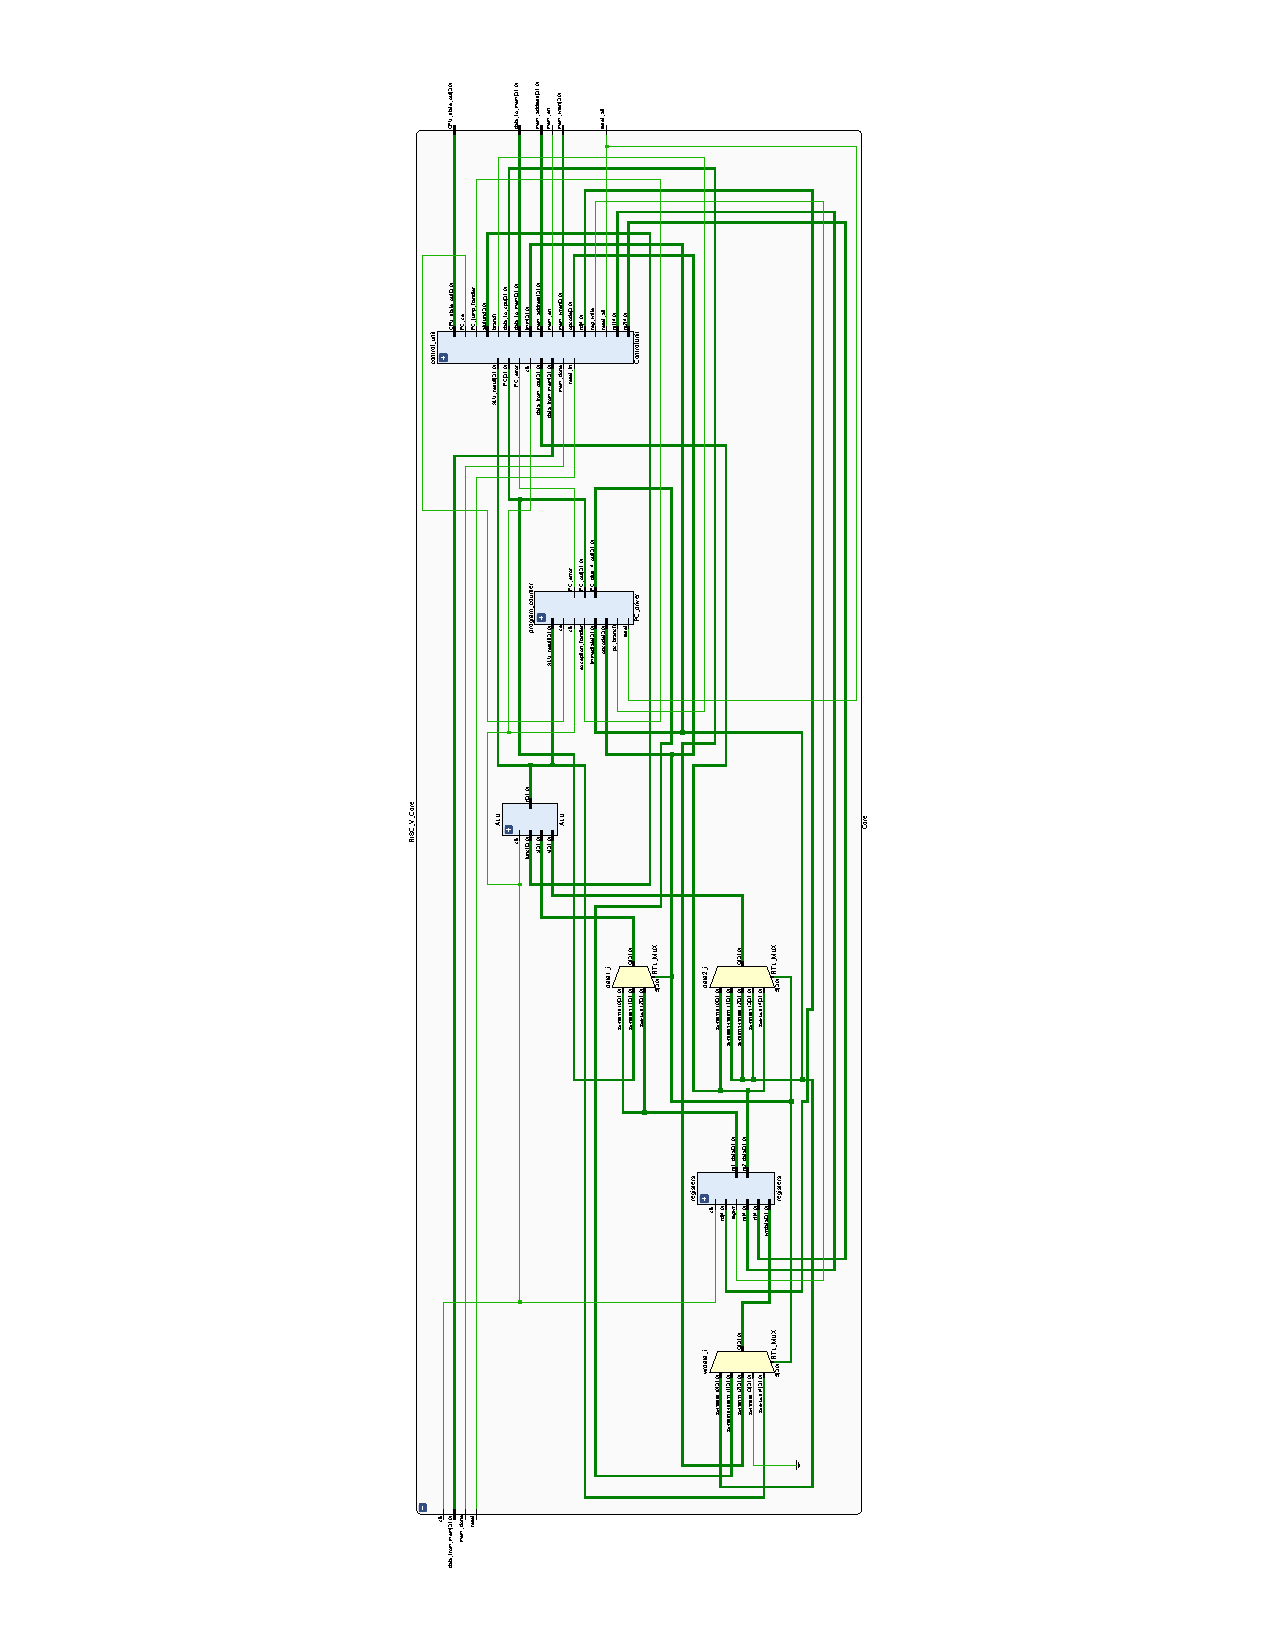
\includepdf[pages=1,scale=0.75,offset=0 -80, pagecommand={
\chapter{Přílohy}
\section{Shéma jádra procesoru RISC-V}
\label{appendix:Core}
\hfill}]{assets/Core_schematic.pdf}

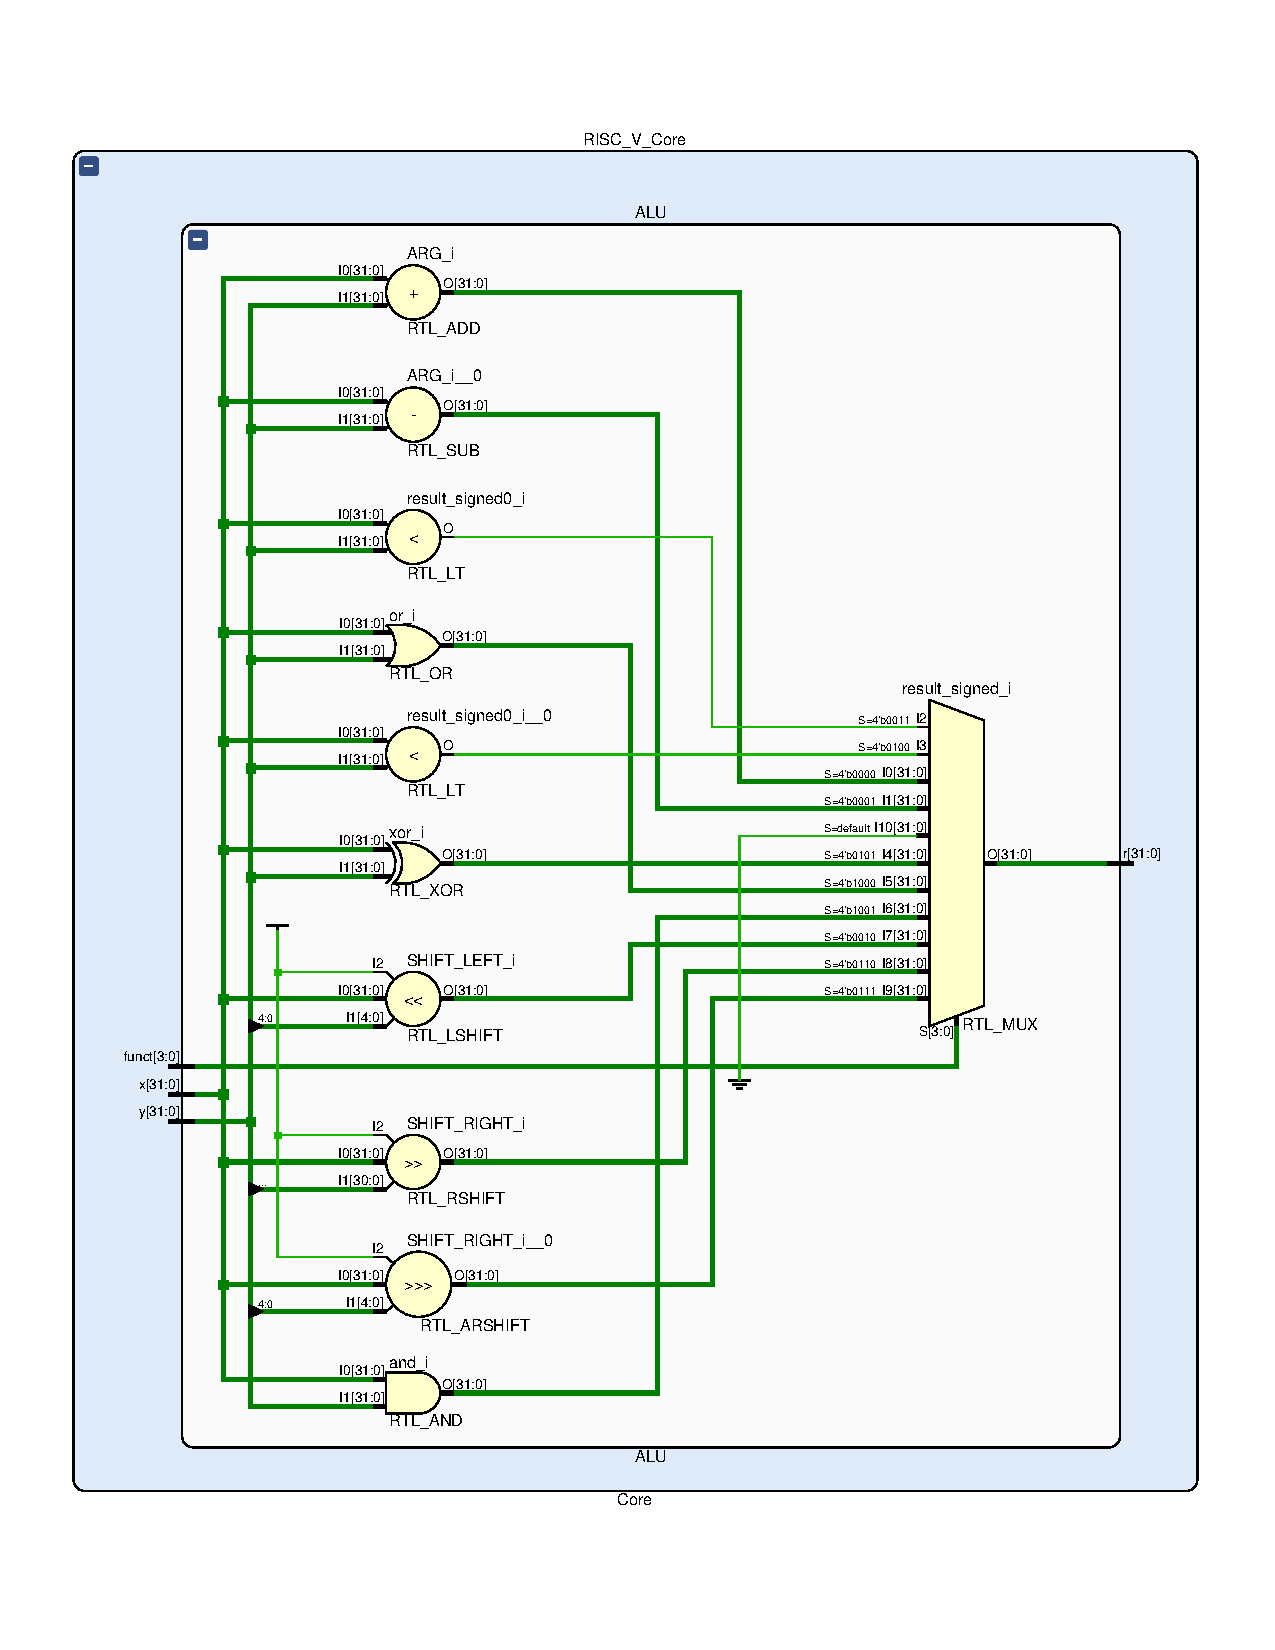
\includepdf[pages=1,scale=0.85,pagecommand={
\section{Shéma ALU}
\label{appendix:ALU}
\hfill}]{assets/ALU_schematic.pdf}

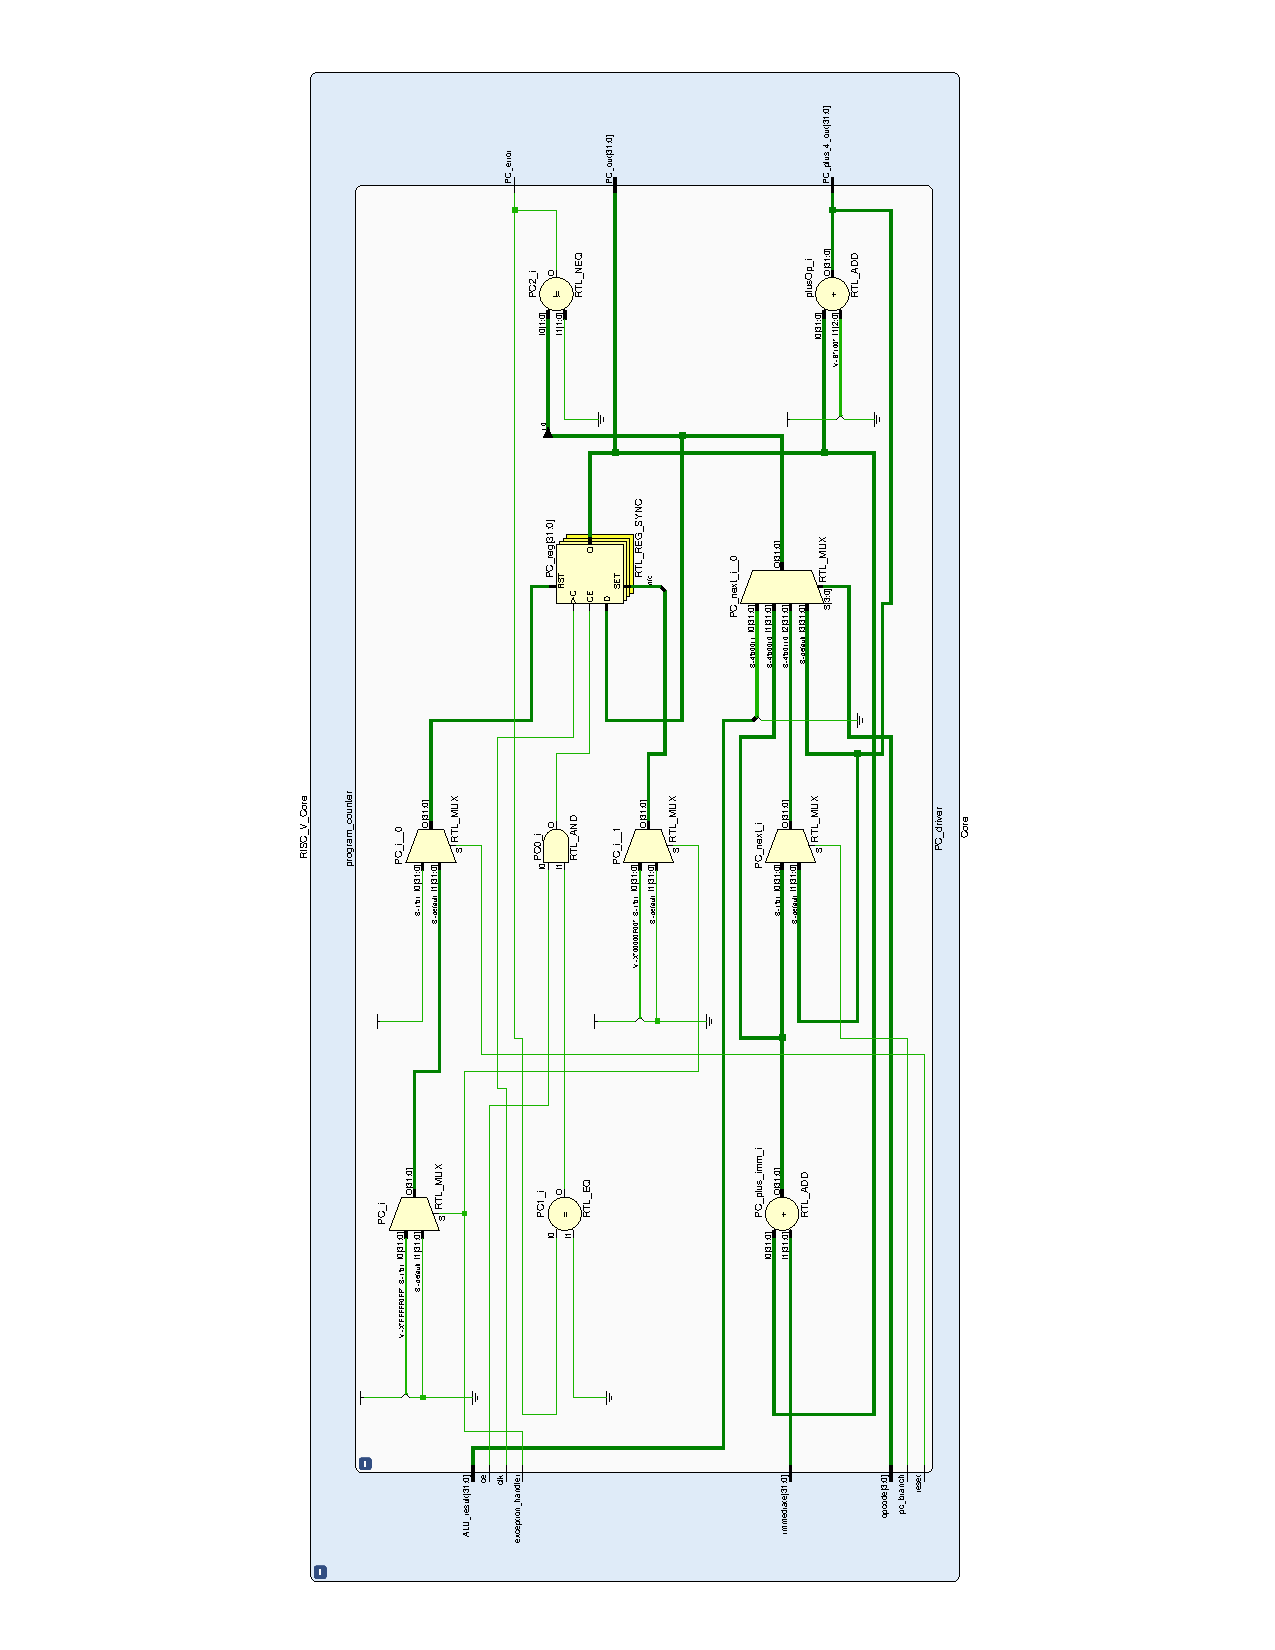
\includepdf[pages=1,scale=0.85,pagecommand={
\section{Shéma čítače instrukcí}
\label{appendix:pc}
\hfill}]{assets/PC_schematic.pdf}

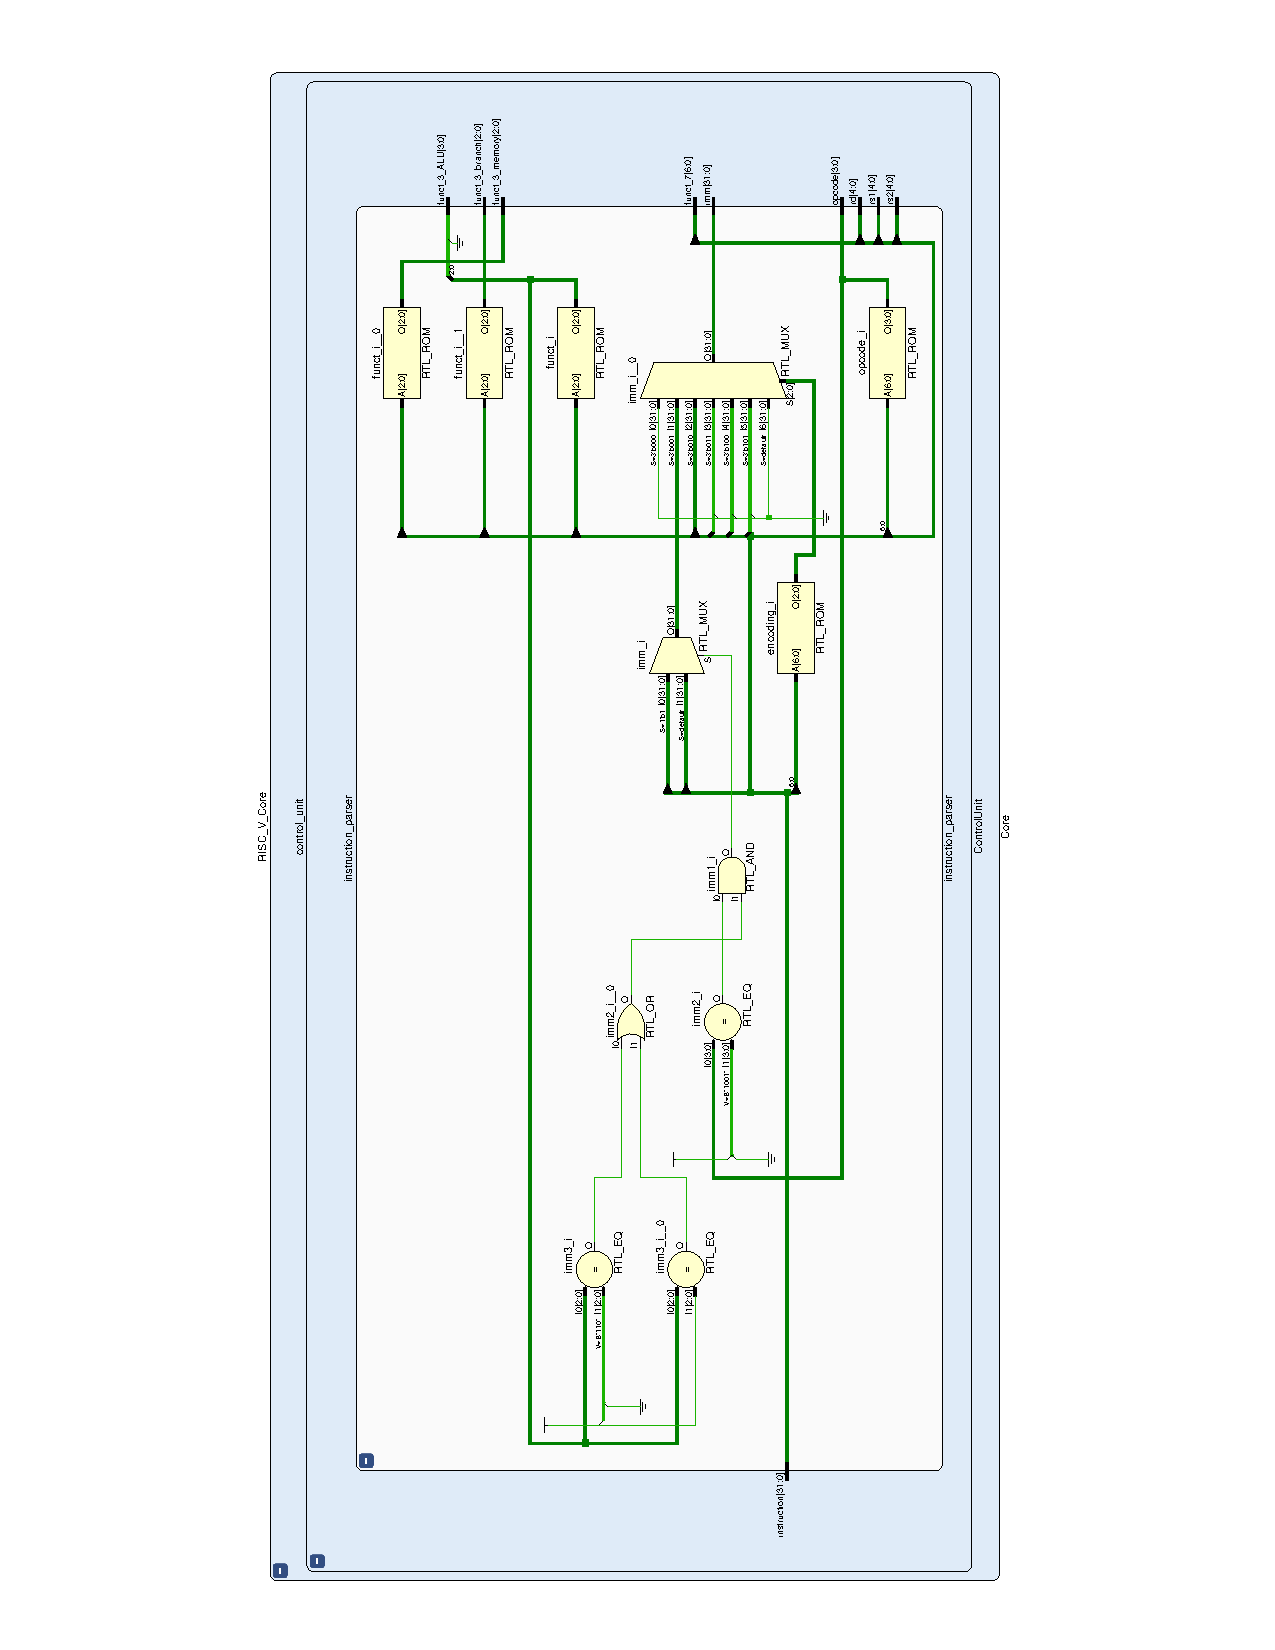
\includepdf[pages=1,scale=0.85,pagecommand={
\section{Shéma dekodéru instrukcí}
\label{appendix:decoder}
\hfill}]{assets/Decoder_schematic.pdf}

\section{Program: Fibonaciho posloupnost v C}
\begin{listing}[h]
    \inputminted[linenos]{c}{assets/fibonaci.c}
    \caption{Fibonaciho posloupnost v jazyce C}
    \label{listing:fib_c}
\end{listing}
\newpage

\section{Program: Fibonaciho posloupnost v assembly}
\inputminted[linenos]{gas}{assets/fib_func.asm}
\begin{listing}[h]
    \caption{Fibonaciho posloupnost v jazyce assembly}
    \label{listing:fib_asm}
\end{listing}

\printbibliography[title={Použitá literatura}] % sazba seznamu citací 
% \printbibliography[title={References}] 
\addcontentsline{toc}{chapter}{Použitá literatura}

\renewcommand{\indexname}{Rejstřík instrukcí a pojmů}
\printindex

\end{document}
